% slide di panoramica sulla tecnologia XML
% % Panoramica XML: definizione, sintassi, documento ben formato, documento valido
% cos'è XML
% XML is used when you want to mark up a textual resource and to store data in a suitable and recognized standard way.

%% slide premesse


\documentclass{beamer}
    
    %    \usepackage[english]{babel}
        %\usepackage[latin1]{inputenc}
        %\usepackage[T1]{fontenc}
    
    \mode<presentation>{
      \setbeamertemplate{background canvas}[vertical shading]
      \usetheme{Berkeley}
      \useoutertheme{himinfolines}
    }
      
    \usepackage{ucs}
    \usepackage[utf8]{inputenc}
    \usepackage[english,polutonikogreek,italian,UKenglish,british]{babel}
    \usepackage{graphicx}
    \usepackage{colortbl}
    \usepackage{multicol}
    \usepackage{ulem}
    \usepackage{verbatim}
    \usepackage{alltt}
    \usepackage{ccicons}
    \usepackage{MnSymbol,wasysym}
    \usepackage{tikzsymbols}
    \usepackage{textcomp}
    \usepackage{xmpincl}
    
    \usepackage{parskip}
    \setcounter{nframes}{100}
    \setcounter{nframe}{1}
    \setbeamercovered{dynamic}
    \newenvironment{grcenv}{\begin{otherlanguage}{greek}}{\end{otherlanguage}}
    \newcommand{\g}[1]{\textgreek{#1}}
    \definecolor{darkgreen}{rgb}{0,0.5,0}
    \definecolor{darkblue}{rgb}{0,0,0.5}
    \definecolor{grey}{rgb}{0.5,0.5,0.5}
    \setcounter{tocdepth}{5}
    
    \makeatletter
    
    \makeatother
    %\includexmp{LicencesAndLicensing}
    
    %frame00 metadata
        \title{Codifica di Testi - XML Schema e Intro TEI \\a.a. 2018-2019}
        \author[A.M. Del Grosso]{Angelo Mario Del Grosso}
        \institute{\texttt{angelo.delgrosso@ilc.cnr.it} \\\bigskip\textit{CNR-ILC-LicoLab}}
        \date{Istituto di Linguistica Computazionale ``A. Zampolli'', \today}
        \AtBeginSection[]{
        \begin{frame}<beamer>
        \addtocounter{nframe}{1}
        \footnotesize
        \frametitle{Progress status}
        \tableofcontents[currentsection,hideothersubsections]
        \end{frame}
        }
    
\begin{document}

\begin{frame}
	\maketitle
\end{frame}

\begin{frame}
	\frametitle{Contenuto della lezione}
	\tableofcontents
\end{frame}

\section{XML Schema Definition (XSD)}
%slide relative ad introdurre gli elementi di XML Schema Definition (XSD) 

%frame 01
\begin{frame}
	\frametitle{Elementi per la definizione degli schemi xml}
	\framesubtitle{principi XML Schema Definition}
	\addtocounter{nframe}{1}

	\begin{block}{Cos'è uno schema XML}
		Uno schema XML è un documento XML standard che descrive come deve essere realizzato un altro documento XML.
		\\ Ci riferiamo a questa tecnologia con l'acronimo XSD.
	\end{block}

	\begin{block}{A cosa serve uno Schema XML}
		I documenti XSD sono usati per validare documenti XML.
		\\ Tuttavia un documento XSD viene realizzato tramite l'uso di un vocabolario predefinito riferibile attraverso un namespace con URI standard.
	\end{block}

\end{frame}

%frame 02
\begin{frame}
	\frametitle{Elementi per la definizione degli schemi xml}
	\framesubtitle{principi XSD}
	\addtocounter{nframe}{1}

	\begin{block}{XSD Schema}
		Il termine XSD o XML Schema denota un documento XML che descrive e valida la struttura e il contenuto di un altro documento XML.
	\end{block}

	\begin{block}{XSD Schema}
		\textbf{Dichiarazione del documento (declaration) e istanza del documento (instance).}
	\end{block}

\end{frame}

%frame 03
\begin{frame}
	\frametitle{Elementi per la definizione degli schemi xml}
	\framesubtitle{principi XSD}
	\addtocounter{nframe}{1}

	\begin{block}{XSD elemento root}
		L'elemento radice di uno schema XSD è sempre l'elemento ``\texttt{<schema>}''.
		\\ Tutte le definizione devono seguire quindi l'elemento ``\texttt{<schema>}''.
	\end{block}

	\begin{block}{XSD Schema}
		Tutti gli elementi e gli attributi dello schema sono dichiarati all'interno del namespace ``\texttt{http://www.w3.org/2001/XMLSchema.}''.
		\\ Tutti i documenti XSD contengono la dichiarazione a questo namespace con prefisso convenzionale \textbf{xsd} oppoure \textbf{xs}.
	\end{block}

\end{frame}

\begin{frame}
	\frametitle{Elementi per la definizione degli schemi xml}
	\framesubtitle{principi XSD}
	\addtocounter{nframe}{1}

	\begin{block}{XSD componenti di base}
		I componenti di base di uno Schema XSD sono le dichiarazioni degli elementi e le dichiarazioni degli attributi.
	\end{block}

	\begin{block}{XSD Schema}
		\textbf{Le dichiarazioni più complesse si poggiano su queste unità: elementi e attributi.}
	\end{block}

\end{frame}

\begin{frame}
	\frametitle{Elementi per la definizione degli schemi xml}
	\framesubtitle{principi XSD}
	\addtocounter{nframe}{1}

	\begin{block}{XSD dichiarazioni}
		Scrivere un pezzo di codice XSD per descrivere e validare un elemento per un documento XML è detto \textit{element declaration}.
	\end{block}

	\begin{block}{XSD dichiarazioni di base}
		XSD permette di dichiarare elementi, attributi e di specificare il numero di figli, le occorrenze, l'ordine di apparizione, e i tipi di dati del content model.
	\end{block}

\end{frame}


\begin{frame}
	\frametitle{Elementi per la definizione degli schemi xml}
	\framesubtitle{principi XSD}
	\addtocounter{nframe}{1}

	\begin{block}{Element Types: simple and complex}
		La dichiarazione di un elemento può avere un tipo semplice (\textit{simple type}) oppure un tipo complesso (\textit{complex type}) a seconda della sua struttura e del suo contenuto.


	\end{block}

	\begin{block}{Simple Type e Complex Type}
		La dichiarazione di un elemento ha un tipo semplice se non possiede \textbf{né figli né attributi}.
		\\ La dichiarazione di un elemento ha un tipo complesso in tutti gli altri casi.
	\end{block}

\end{frame}


%frame 04
\begin{frame}
	\frametitle{Elementi per la definizione degli schemi xml}
	\framesubtitle{principi XSD}
	\addtocounter{nframe}{1}

	%\defverbatim{\xsdfirst}{%
	%\begin{tiny}
	%\begin{verbatim}
	%    <xsd:schema xmlns:xsd="http://www.w3.org/2001/XMLSchema">
	%        <xsd:element name="text"/>
	%    </xsd:schema>
	%\end{verbatim}
	%    \end{tiny}
	%   }

	%  \defverbatim{\xmlfirst}{%
	% \begin{tiny}
	%\begin{verbatim}
	%         <text>Il primo documento XML Validato</text>
	% \end{verbatim}
	% \end{tiny}
	% }


	\begin{block}{XSD esempio}
		% {\xsdfirst}
		\texttt{<xsd:schema xmlns:xsd=``http://www.w3.org/2001/XMLSchema''>}
		\\\texttt{<xsd:element name=``text''/>}
		\\\texttt{</xsd:schema>}
	\end{block}

	\begin{block}{XSD esempio elemento di tipo semplice}
		% {\xsdfirst}
		\texttt{<text>Il primo documento XML Validato</text>}
	\end{block}



\end{frame}

\begin{frame}
	\frametitle{Elementi per la definizione degli schemi xml}
	\framesubtitle{principi XSD}
	\addtocounter{nframe}{1}

	\begin{block}{XML XSD esempio}
		Il documento XML istanza dello schema XSD per essere valido deve contenere un elemento radice.
		Validare il documento XML con il relativo XSD con XMLlint.

	\end{block}

	\begin{block}{XMLlint}
		\texttt{xmllint xmlfirst.xml --schema ../schema/xsd/xsdfirst.xsd}
	\end{block}


\end{frame}

\begin{frame}
	\frametitle{Elementi per la definizione degli schemi xml}
	\framesubtitle{principi XSD}
	\addtocounter{nframe}{1}

	\begin{block}{Element Complex Types: esempio}

		%If an element contains child elements or attributes, it has a complex type.
		\texttt{
			<xsd:schema xmlns:xsd=``http://www.w3.org/2001/XMLSchema''>
			<xsd:element name=``Employee''>
			<xsd:complexType>
			<xsd:attribute name=``FirstName''/>
			</xsd:complexType>
			</xsd:element>
			</xsd:schema>
		}
	\end{block}

	\begin{block}{Element Complex Types: esempio}
		Il documento XML istanza dello schema:
		\\\texttt{<Employee FirstName="Jacob"/>}
	\end{block}

\end{frame}

\begin{frame}
	\frametitle{Elementi per la definizione degli schemi xml}
	\framesubtitle{principi XSD}
	\addtocounter{nframe}{1}

	\begin{block}{Complex Types}
		Alla base dello standard XSD ci sono le dichiarazioni degli elementi e degli attributi, ad un livello di astrazione più alto ci sono i types e i groups.

	\end{block}

	\begin{block}{Element Complex Types}
		\textbf{Un tipo complesso (Complex Type) può avere attributi e/o elementi figli.}
	\end{block}

\end{frame}

\begin{frame}
	\frametitle{Elementi per la definizione degli schemi xml}
	\framesubtitle{principi XSD}
	\addtocounter{nframe}{1}

	\begin{block}{Element Complex Types: Esempio Elemento con Figlio}
		\texttt{
			<xsd:schema xmlns:xsd=``http://www.w3.org/2001/XMLSchema''>
			<xsd:element name=``text''>
			<xsd:complexType>
			<xsd:sequence>
			<xsd:element name=``body''/>
			</xsd:sequence>
			</xsd:complexType>
			</xsd:element>
			</xsd:schema>}
	\end{block}

\end{frame}


\begin{frame}
	\frametitle{Elementi per la definizione degli schemi xml}
	\framesubtitle{principi XSD}
	\addtocounter{nframe}{1}

	\begin{block}{Espressività dell'XSD}

		\begin{itemize}
			\item Attribute Group, Element Group
			\item Order Indicators: all, sequence, choice
			\item Occurrence Indicators: minOccurs and maxOccurrs
			\item Annotation (utili per documentare le dichiarazioni)
		\end{itemize}

	\end{block}

\end{frame}

\begin{frame}
	\frametitle{Elementi per la definizione degli schemi xml}
	\framesubtitle{principi XSD}
	\addtocounter{nframe}{1}

	\begin{block}{Espressività dell'XSD}
		\begin{itemize}
			\item Data types: Built-in
			\item FACETS per una validazione oculata dei valori (elemento o un attributo).
			\item Restriction on base attribute
			\item Numeric e String Data Type
			\item Pattern facet
		\end{itemize}

	\end{block}

\end{frame}


\begin{frame}
	\frametitle{Elementi per la definizione degli schemi xml}
	\framesubtitle{principi XSD}
	\addtocounter{nframe}{1}

	\begin{block}{Element Declaration}
		Una dichiarazione di elemento (\textbf{XSD element declaration}) rappresenta un elemento nel documento XML istanza dello schema. 
		
	\end{block}

	\begin{block}{Element Declaration: Istanza XML }
		\texttt{<p>il contentuto testuale di un paragrafo</p>}
	\end{block}
	\textit{Un elemento ha un tipo semplice (\textbf{simple type}) se non ha attributi e non ha elementi figli}
\end{frame}


%% An XSD schema may contain Global and Local element declarations.

\begin{frame}
	\frametitle{Elementi per la definizione degli schemi xml}
	\framesubtitle{principi XSD}
	\addtocounter{nframe}{1}

	\begin{block}{Global and Local element declaration}
		Il vantaggio di usare dichiarazioni di elementi globali (\textbf{global element declaration})
		è che la dichiarazione può essere riferita più volte da altre dichiarazioni all'interno del documento XSD.
	\end{block}

\end{frame}


\begin{frame}
	\frametitle{Elementi per la definizione degli schemi xml}
	\framesubtitle{principi XSD}
	\addtocounter{nframe}{1}

	\begin{block}{Global element declaration: esempio}
		\texttt{<xsd:schema xmlns:xsd=``http://www.w3.org/2001/XMLSchema">
			\emph{<xsd:element name=``body''>}
			<xsd:complexType>
			<xsd:attribute name=``lang''/>
			<xsd:attribute name=``type''/>
			</xsd:complexType>
			</xsd:element>
			<xsd:element name=``text''>
			<xsd:complexType>
			<xsd:all>
			\emph{<xsd:element ref=``body''/>}
			</xsd:all>
			</xsd:complexType>
			</xsd:element>
			</xsd:schema>}
	\end{block}

\end{frame}


\begin{frame}
	\frametitle{Elementi per la definizione degli schemi xml}
	\framesubtitle{principi XSD}
	\addtocounter{nframe}{1}

	\begin{block}{Group declaration}
		Attributi e elementi possono essere raggruppati in costrutti detti \textbf{Attribute Groups} e \textbf{Element Groups}.
	\end{block}
	
	\textit{E' possibile riferirsi a questi gruppi all'interno di altre dichiarazioni ottenendo un significativo grado di riusabilità.}

\end{frame}


\begin{frame}
	\frametitle{Elementi per la definizione degli schemi xml}
	\framesubtitle{principi XSD}
	\addtocounter{nframe}{1}


	\begin{block}{Global element declaration: esempio}
		\texttt{\emph{<xsd:group name=``fileDesc''>}
			<xsd:sequence>
			<xsd:element name=``titleStmt''/>
			<xsd:element name=``publicationStmt''/>
			<xsd:element name=``sourceDesc''/>
			</xsd:sequence>
		}
	\end{block}

	\begin{block}{Global element declaration: esempio}
		\begin{center} \texttt{<xsd:group ref=``fileDesc''/>}\end{center}
	\end{block}

\end{frame}

\begin{frame}
	\frametitle{Elementi per la definizione degli schemi xml}
	\framesubtitle{principi XSD}
	\addtocounter{nframe}{1}

	\begin{block}{Element Declaration: Attributi nella dichiarazione}
		L'unico attributo \textit{obbligatorio} nella dichiarazione di elementi è l'attributo \textbf{name}.
	\end{block}

	\begin{block}{Element Declaration: Attributi - Esempio}
		\begin{center}\texttt{<xsd:element name=``TEI''/> }\end{center}
	\end{block}

\end{frame}

\begin{frame}
	\frametitle{Elementi per la definizione degli schemi xml}
	\framesubtitle{principi XSD}
	\addtocounter{nframe}{1}

	\begin{block}{Element declaration: lista Attributi}
		\begin{itemize}
			\item \textbf{name} (\textit{g-l}): il nome dell'elemento, unico attributo obbligatorio (\textit{dare nomi significativi agli elmenti})
			\item \textbf{type} (\textit{g-l}): aggiunta di un tipo di dato (\textit{data type}) (XSD ha buint-in data types)
			\item \textbf{id} (\textit{g-l}): identificatore univoco della dichiarazione dell'elemento(non ha effetti sull'istanza XML)
			\item \textbf{default} (\textit{g-l}): spcifica il valore di default di un elemento (solo se l'elemento è opzionale)
		\end{itemize}

	\end{block}

\end{frame}

\begin{frame}
	\frametitle{Elementi per la definizione degli schemi xml}
	\framesubtitle{principi XSD}
	\addtocounter{nframe}{1}

	\begin{block}{Element declaration: lista Attributi (cont.)}
		\begin{itemize}
			\item \textbf{fixed} (\textit{g-l}): valore di un elemento predefinito (``fixed'' e ``default'' sono mutuamente esclusivi)
			\item \textbf{nillable} (\textit{g-l}): indica che l'elemento è vuoto (xsd:nil nell'istanza XML del documento)
			\item \textbf{block} (\textit{g-l}): è utilizzato per controllare la sostizione degli elementi ( può assumere 4 differenti valori: \textit{substitution}, \textit{extension} \textit{restriction} e \textit{\#all})
		\end{itemize}
	\end{block}

\end{frame}

\begin{frame}
	\frametitle{Elementi per la definizione degli schemi xml}
	\framesubtitle{principi XSD}
	\addtocounter{nframe}{1}

	\begin{block}{Element declaration: lista Attributi (cont.)}

		\begin{itemize}
			\item \textbf{final} (\textit{g}): limita la dichiarazione dei gruppi di sostituzione ( può assumere 3 valori: \textit{\#all}, \textit{restriction} and \textit{extension})
			\item \textbf{abstract} (\textit{g}): un elemento astratto non può essere istanziato (è un modo per forzare la sostituzione)
			\item \textbf{substitutionGroup} (\textit{g}): è un modo per avere grande estensibilità delle dichiarazioni (facilità la creazione di nuovi tipi di elementi derivati)
			\item \textbf{minOccurs} (\textit{l}): controlla il numero di occorrenze minime degli elementi all'interno del documento XML istanza dello schema. (\textbf{minOccurs=0} indica elemento \textit{optionale}).
		\end{itemize}
	\end{block}

\end{frame}

\begin{frame}
	\frametitle{Elementi per la definizione degli schemi xml}
	\framesubtitle{principi XSD}
	\addtocounter{nframe}{1}

	\begin{block}{Element declaration: lista Attributi (cont.)}

		\begin{itemize}
			\item \textbf{maxOccurs} (\textit{l}): controlla il numero massimo di occorrenze degli elementi all'interno del documento XML istanza dello schema
			\item \textbf{ref} (\textit{l}): riferimento ad altri elementi dichiarati globalmente all'interno dello schema (riusabilità)
			\item \textbf{form} (\textit{l}): specifica se l'elemento deve essere qualificato con l'aggiunta del namespace (``qualified'' oppure ``unqualified'').
		\end{itemize}
	\end{block}

\end{frame}

\begin{frame}
	\frametitle{Elementi per la definizione degli schemi xml}
	\framesubtitle{principi XSD}
	\addtocounter{nframe}{1}

	\begin{block}{Element declaration: Attributi - Esempio }

		\texttt{
			<xsd:element name=``body''>
			<xsd:complexType>
			\emph{<xsd:sequence maxOccurs=``unbounded''>}
			\emph{<xsd:element ref=``div''/>}
			</xsd:sequence>
			</xsd:complexType>
			</xsd:element>
		}

	\end{block}


	\begin{block}{Element declaration: Attributi - Esempio }

		\texttt{
			<xsd:element name=``div'' type=``divType'' />
		}
		\texttt{
			<xsd:complexType name=``divType''>
			[...]
			</xsd:complexType>
		}

	\end{block}

\end{frame}

% fare un paio di slide spiegando a cosa serve l'attribute substitutionGroup e come si usa. (pp 114-133)

% The substitutionGroup attribute is used to declare elements capable of
%serving as variable content containers. Abstract is used to specify that the
%element cannot be instantiated directly. To instantiate such an element, a
%substitution element needs to be created. The block and final attributes are
%used to control substitution of the element. Final restricts substitution at
%schema level and block restricts it at instance level.


% Attribute Declaration
% simple example
% <xsd:schema xmlns:xsd="http://www.w3.org/2001/XMLSchema">
%   <xsd:element name="Employee">
%     <xsd:complexType>
%       <xsd:attribute name="status" />
%     </xsd:complexType>
%   </xsd:element>
% </xsd:schema>



\begin{frame}
	\frametitle{Elementi per la definizione degli schemi xml}
	\framesubtitle{principi XSD}
	\addtocounter{nframe}{1}

	\begin{block}{Attribute declaration}
		Un attributo è dichiarato utilizzando l'elemento \texttt{<xsd:attribute>}. \\ L'unico attributo obbligatorio nella dichiarazione è ``\textbf{name}''.
	\end{block}

	\begin{block}{Attribute declaration: Global vs Local}
		Quando una dichiarazione di attributo ha il livello gerarchico successivo a ``\texttt{<xsd:schema>}'' (\textit{la root dello schema}), questa dichiarazione è detta globale (\textit{global attribute declaration}. In caso contrario l'attributo è all'interno di un \textit{Complex Type}, ed è una (\textit{Local attribute declaration}).
	\end{block}

\end{frame}

\begin{frame}
	\frametitle{Elementi per la definizione degli schemi xml}
	\framesubtitle{principi XSD}
	\addtocounter{nframe}{1}
	\begin{block}{Attribute declaration}

		\texttt{
			<xsd:attribute name=``Name'' type=``xsd:string''/>
		}

	\end{block}
	\textit{Qualsiasi dichiarazione di attributo per essere effettivamente utile deve essere riportata all'interno di una dichiarazione di elemento}
\end{frame}

% tabella con gli attributi nella dichiarazione degli attributi
% "attributes of an attribute declaration"

\begin{frame}
	\frametitle{Elementi per la definizione degli schemi xml}
	\framesubtitle{principi XSD}
	\addtocounter{nframe}{1}

	\begin{block}{Attribute declaration: Attributi}
		\begin{itemize}
			\item \textbf{name} (\textit{g-l}): il nome dell'attributo, attributo obbligatorio.
			\item \textbf{id} (\textit{g-l}): l'identificativo della dichiarazione all'interno del documento XSD (non influenza l'istanza XML).
			\item \textbf{type} (\textit{g-l}): associa un tipo di dato allo spazio di valori che può assumere l'attributo.
		\end{itemize}

	\end{block}

\end{frame}


\begin{frame}
	\frametitle{Elementi per la definizione degli schemi xml}
	\framesubtitle{principi XSD}
	\addtocounter{nframe}{1}

	\begin{block}{Attribute declaration: Attributi (cont.)}
		\begin{itemize}
			\item \textbf{default} (\textit{g-l}): assegna un valore di default all'attributo (solo se l'attributo non è presente).
			\item \textbf{fixed} (\textit{g-l}): assegna un valore predefino e fisso all'attributo.
			\item \textbf{ref} (\textit{l}): riferimento ad una dichirazione di attributo globale
		\end{itemize}
	\end{block}


\end{frame}


\begin{frame}
	\frametitle{Elementi per la definizione degli schemi xml}
	\framesubtitle{principi XSD}
	\addtocounter{nframe}{1}

	\begin{block}{Attribute declaration: Attributi (cont.)}
		\begin{itemize}
			\item \textbf{use} (\textit{l}): specifica se l'attributo è opzionale o meno. Possibili valori sono \textit{optional}, \textit{required}, \textit{prohibited}
			\item \textbf{form} (\textit{l}): indica se l'attributo deve avere o meno indicato il namespace all'interno del documento XML istanza dello schema (può assumere due valori: \textit{qualified} e \textit{unqualified})
		\end{itemize}

	\end{block}

\end{frame}


\begin{frame}
	\frametitle{Elementi per la definizione degli schemi xml}
	\framesubtitle{principi XSD}
	\addtocounter{nframe}{1}

	\begin{block}{Attribute declaration: Esempio (global)}

		\texttt{
			<xsd:schema xmlns:xsd=``http://www.w3.org/2001/XMLSchema''>
			\emph{<xsd:attribute name=``analysis'' />}
			<!-- -->
			<xsd:element name=``word''>
			<xsd:complexType>
			\emph{<xsd:attribute ref=``analysis''/>}
			</xsd:complexType>
			</xsd:element>
			</xsd:schema>
		}

	\end{block}

	\textit{Global attribute declarations are useful when an attribute is declared with several validations}


\end{frame}



%% Esempio da img GlobalAttribute
%% global attribute declarations provide some sort of re-usability.

%% esempio type:
% <xsd:schema xmlns:xsd="http://www.w3.org/2001/XMLSchema">
%   <xsd:element name="Employee">
%     <xsd:complexType>
%       <xsd:attribute name="Age" type="xsd:positiveInteger"/>
%     </xsd:complexType>
%   </xsd:element>
% </xsd:schema>

%% Attribute Groups
% Attribute Groups provide a convenient means to reuse attribute declarations in multiple complex types. Attribute Groups provide a better level of reusability by grouping one or more attribute declarations into a named group. By using an attribute group, you can avoid this repetition of code. Chain of attribute group hierarchies.

\begin{frame}
	\frametitle{Elementi per la definizione degli schemi xml}
	\framesubtitle{principi XSD}
	\addtocounter{nframe}{1}

	\begin{block}{Attribute declaration: Attribute Groups}
		Definire gruppi di attributi permette di riusare le dichirazioni degli attributi in molteplici altre dichiarazioni all'interno dello schema.
		\\I gruppi di attributi permettono di avere un maggiore livello di riusabilità delle dichiarazioni.
	\end{block}

	\textit{Attraverso l'uso dei gruppi di attributi si evitano inutili ripetizioni nel codice XSD ed è possibile costruire catene di gruppi strutturate in gerarchie ben controllate}
\end{frame}


\begin{frame}
	\frametitle{Elementi per la definizione degli schemi xml}
	\framesubtitle{principi XSD}
	\addtocounter{nframe}{1}

	\begin{block}{Attribute declaration: Esercizio (global)}
		\texttt{
			%<xsd:schema xmlns:xsd=``http://www.w3.org/2001/XMLSchema''>
			<xsd:attributeGroup name=``EmpAttributes''>
			%<!-- Declaration of attribute ``name'' -->
			<xsd:attribute name=``name''>
			<xsd:simpleType>
			<xsd:restriction base=``xsd:string''>
			<xsd:maxLength value=``20''/>
			</xsd:restriction>
			</xsd:simpleType>
			</xsd:attribute>
			%<!-- Declaration of attribute ``department'' -->
			<xsd:attribute name=``department''>
			<xsd:simpleType>
			<xsd:restriction base=``xsd:string''>
			<xsd:length value=``2''/>
			</xsd:restriction>
			</xsd:simpleType>
			</xsd:attribute>
			</xsd:attributeGroup>
			%[...]
		}
	\end{block}

\end{frame}


\begin{frame}
	\frametitle{Elementi per la definizione degli schemi xml}
	\framesubtitle{principi XSD}
	\addtocounter{nframe}{1}

	\begin{block}{Attribute declaration: Esercizio (global)}
		\texttt{
			%[...]
			%<!-- Declaration of root element ``Employees'' -->
			<xsd:element name=``Employees''>
			<xsd:complexType>
			<xsd:sequence>
			%<!-- Declaration of ``Manager'' element -->
			<xsd:element name=``Manager''>
			<xsd:complexType>
			<xsd:attributeGroup ref=``EmpAttributes''/>
			</xsd:complexType>
			</xsd:element>
			%<!-- Declaration of ``department'' element -->
			<xsd:element name=``TechLead''>
			<xsd:complexType>
			<xsd:attributeGroup ref=``EmpAttributes''/>
			</xsd:complexType>
			</xsd:element>
			</xsd:sequence>
			</xsd:complexType>
			</xsd:element>
			%</xsd:schema>
		}
	\end{block}

\end{frame}

%% Data type

\begin{frame}
	\frametitle{Elementi per la definizione degli schemi xml}
	\framesubtitle{principi XSD}
	\addtocounter{nframe}{1}

	\begin{block}{XSD Data Type}
		I linguaggi di programmazione uso i tipi (\textit{data types}) per controllare i valori che può assumere una variabile e le operazioni che possono essere effettuate su quest'ultime.
	\end{block}

		\textit{In parole povere, quando si associa un data type ad una variabile si vuole restringere lo spazio di valori permesso e restringere le operazioni che possono elaborare tali valori.}
	

\end{frame}

\begin{frame}
	\frametitle{Elementi per la definizione degli schemi xml}
	\framesubtitle{principi XSD}
	\addtocounter{nframe}{1}

	\begin{block}{XSD Data Type: esempio -  dichiarazione}
		\texttt{
			<xsd:element name=``div''>
			<xsd:complexType>
			\textit{<xsd:attribute name=``type'' />}
			\emph{<xsd:attribute name=``n'' type=``xsd:integer''/>}
			</xsd:complexType>
			</xsd:element>
		}


	\end{block}

	\begin{block}{XSD Data Type: esempio - istanza}
		\texttt{<div type="chapter" n="1" />'} \textit{(corretto)}
		\\\texttt{<div type="chapter" n="uno" />'} \textit{(errato)}

	\end{block}



\end{frame}

\begin{frame}
	\frametitle{Elementi per la definizione degli schemi xml}
	\framesubtitle{principi XSD}
	\addtocounter{nframe}{1}

	\begin{block}{XSD Data Type}
		XSD supporta diversi tipi di dati, per descrivere e validare quasi tutti i valori che possono occorrere in un documento XML. 
		\\\textbf{Ma supporta anche la possibilità di derivare nuovi data types a partire da quelli disponibili (\textit{built-in}}
	\end{block}

	\begin{block}{XSD Data Type}
		I tipi di dati aiutano a descrivere un certo dato in modo più accurato, contribuendo a validarne i valori in modo più efficace.
	\end{block}
	
\end{frame}

\begin{frame}
	\frametitle{Elementi per la definizione degli schemi xml}
	\framesubtitle{principi XSD}
	\addtocounter{nframe}{1}

	\begin{block}{XSD Data Type}
		\textbf{XSD supporta una \textit{cinquantina} di tipi di dato divisi in due categorie: \textit{Primitive Data Types} e \textit{Derived Data Types}.}
	\end{block}
	
\end{frame}

\begin{frame}
	\frametitle{Elementi per la definizione degli schemi xml}
	\framesubtitle{principi XSD}
	\addtocounter{nframe}{1}

	\begin{block}{Primitive Data Types}
		Primitive Data Types sono tipi di dati dai quali sono stati derivati altri tipi di dati.
	\end{block}
	%\textit{XSD has nineteen primitive data types}


	\begin{block}{Primiteive Data Types}

		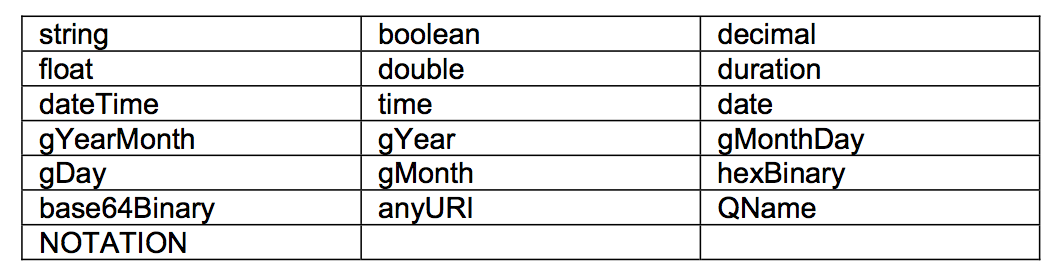
\includegraphics[width=.95\textwidth]{imgs/TabellaDataTypeXSD.png}

	\end{block}

\end{frame}

\begin{frame}
	\frametitle{Elementi per la definizione degli schemi xml}
	\framesubtitle{principi XSD}
	\addtocounter{nframe}{1}

	\begin{block}{Primitive Data Types}
		Primitive Data Types non derivano da alcun tipo di base.
	\end{block}

	\begin{block}{Derived Data Types}

		Nel sistema di tipi di XSD esistono data types che sono direttamente oppure indirettamente derivati dai Primitive Data Types.

	\end{block}

\end{frame}


\begin{frame}
	\frametitle{Elementi per la definizione degli schemi xml}
	\framesubtitle{principi XSD}
	\addtocounter{nframe}{1}

	\begin{center}
		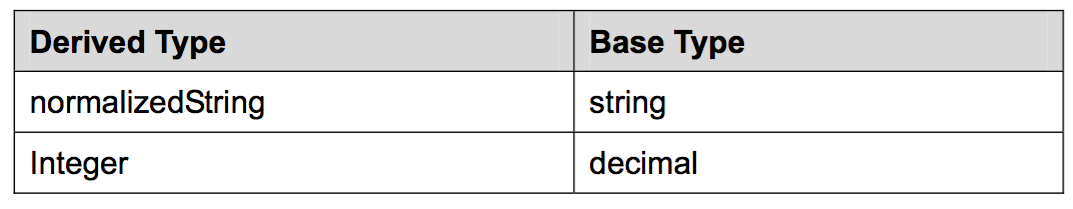
\includegraphics[width=.95\textwidth]{imgs/DerivedTypeBaseType(2types).png}
	\end{center}
	\begin{center}
		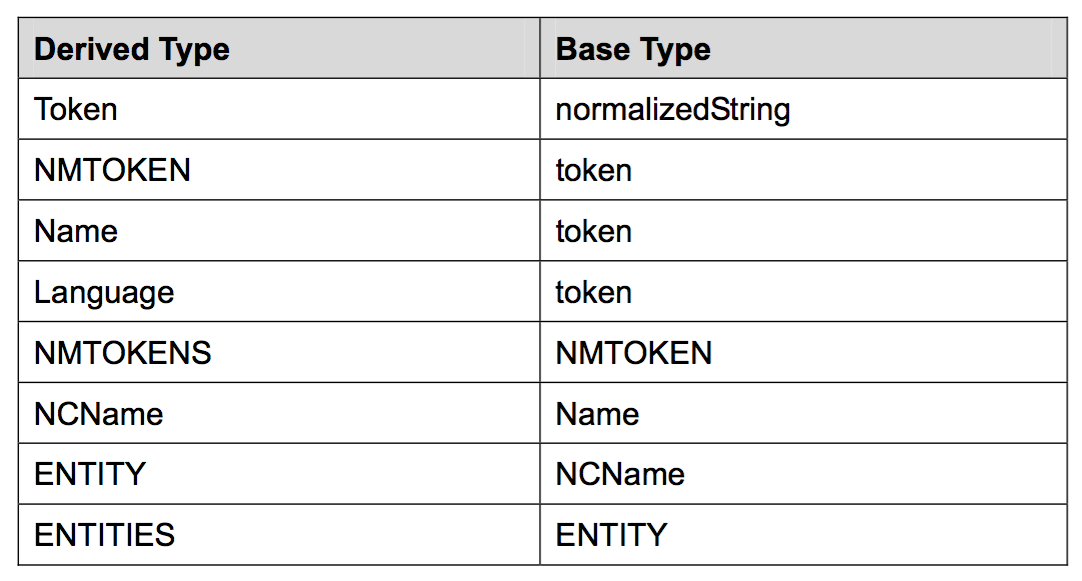
\includegraphics[width=.95\textwidth]{imgs/DerivedTypeFromDerivedType(8types).png}
	\end{center}

\end{frame}

\begin{frame}
	\frametitle{Elementi per la definizione degli schemi xml}
	\framesubtitle{principi XSD}
	\addtocounter{nframe}{1}

	\begin{center}
		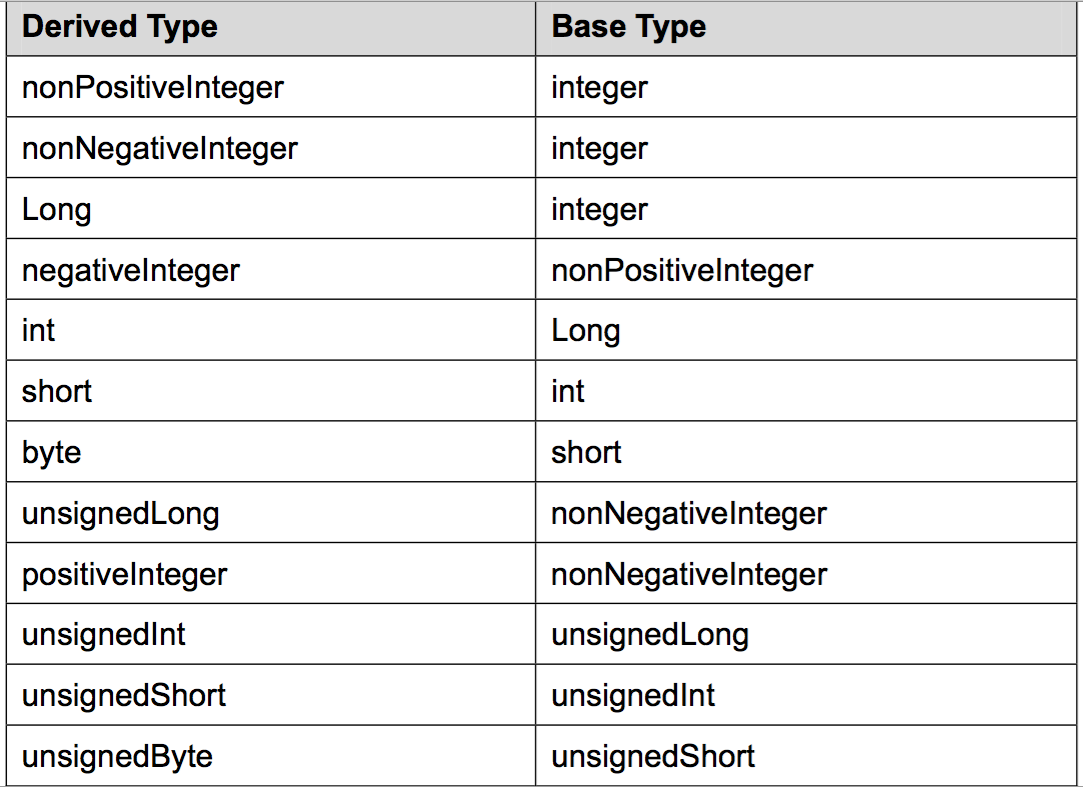
\includegraphics[width=.95\textwidth]{imgs/NumericalDerivedType(12types).png}
	\end{center}

\end{frame}



%% qualche esempio di DataType (libro XSD pagine 175 et seguenti)
% String
% Boolean
% Decimal
%% XSD decimal data type represents a subset of real numbers
% Float
%% XSD float data type is single precision 32-bit floating point type
% Double
%% XSD double data type shares the same characteristics as float except that double data type is double precision 64-bit floating point type.
% Duration
%% XSD duration data type represents duration of time
%% A duration value should always start with the letter "P" in upper case. Then each value should be separated by indicators Y (Years), M (Months), D (Days), H (Hours), M (Minutes) and S (Seconds). Letter "T" should appear as a separator between Year-Month-Day and Hour-Minute-Second.
%% esempio:
% <ElapsedTime>PT3M15S</ElapsedTime>
% DataTime
%% The format of XSD dateTime is -yyyy-mm-ddThh:mm:ss.sZ. 
% hexBinary
%% XSD hexBinary data type represents HEX encoded data.
% "This is a secret message" using the online Text-to- Hex tool available at http://tools.elitehackers.info/Hex.php.
% base64Binary
%% XSD base64Binary data type represents base64 encoded data. store binary data
%% esempio https://www.base64decode.org/
%% VGhpcyBpcyBhIHNlY3JldCBtZXNzYWdl
% QName
%% QName data type can accept a colonized value (a namespace prefix and a string value separated by a colon) only if there is a valid namespace declaration within the scope where the value is used.



\begin{frame}
	\frametitle{Elementi per la definizione degli schemi xml}
	\framesubtitle{principi XSD}
	\addtocounter{nframe}{1}

	\begin{block}{Data Type: Facets}
		Ciascun tipo di dato a una collezione di proprietà che possono essere musate per attuare validazioni aggiuntive ai valori permessi dal tipo di dato corrente.
		\\\textit{Queste proprietà sono chiamate \textbf{Facets} in XSD.}
	\end{block}

	\begin{block}{Data Type: Facets}
		Ogni tipo ha un insieme stabilito di Facets che controllano una certa proprietà o una certa caratteristica del tipo di dato considerato.
	\end{block}

\end{frame}

\begin{frame}
	\frametitle{Elementi per la definizione degli schemi xml}
	\framesubtitle{principi XSD}
	\addtocounter{nframe}{1}

	\begin{block}{Data Type: Facets Esempio}
		\texttt{
			%<xsd:schema xmlns:xsd=``http://www.w3.org/2001/XMLSchema''>
			<xsd:element name=``name''>
			<xsd:complexType>
			<xsd:attribute name=``type''>
			<xsd:simpleType>
			\emph{<xsd:restriction base=``xsd:string''>}
			\emph{<xsd:length value=``15''/>}
			</xsd:restriction>
			</xsd:simpleType>
			</xsd:attribute>
			</xsd:complexType>
			</xsd:element>
			%</xsd:schema>
		}

	\end{block}

\end{frame}

\begin{frame}
	\frametitle{Elementi per la definizione degli schemi xml}
	\framesubtitle{principi XSD}
	\addtocounter{nframe}{1}

	\begin{block}{Data Type: Facets Esempio}
		\texttt{
		%<xsd:schema xmlns:xsd=``http://www.w3.org/2001/XMLSchema''>
		<xsd:element name=``name''>
		<xsd:complexType>
		<xsd:attribute name=``type''>
		<xsd:simpleType>
		\emph{<xsd:restriction base=``xsd:string''>}
		\emph{<xsd:pattern value=``[A-Za-z]+''/>}
		</xsd:restriction>
		</xsd:simpleType>
		</xsd:attribute>
		</xsd:complexType>
		</xsd:element>
		%</xsd:schema>
		}

	\end{block}

\end{frame}

\begin{frame}
	\frametitle{Elementi per la definizione degli schemi xml}
	\framesubtitle{principi XSD}
	\addtocounter{nframe}{1}

	\begin{center}
		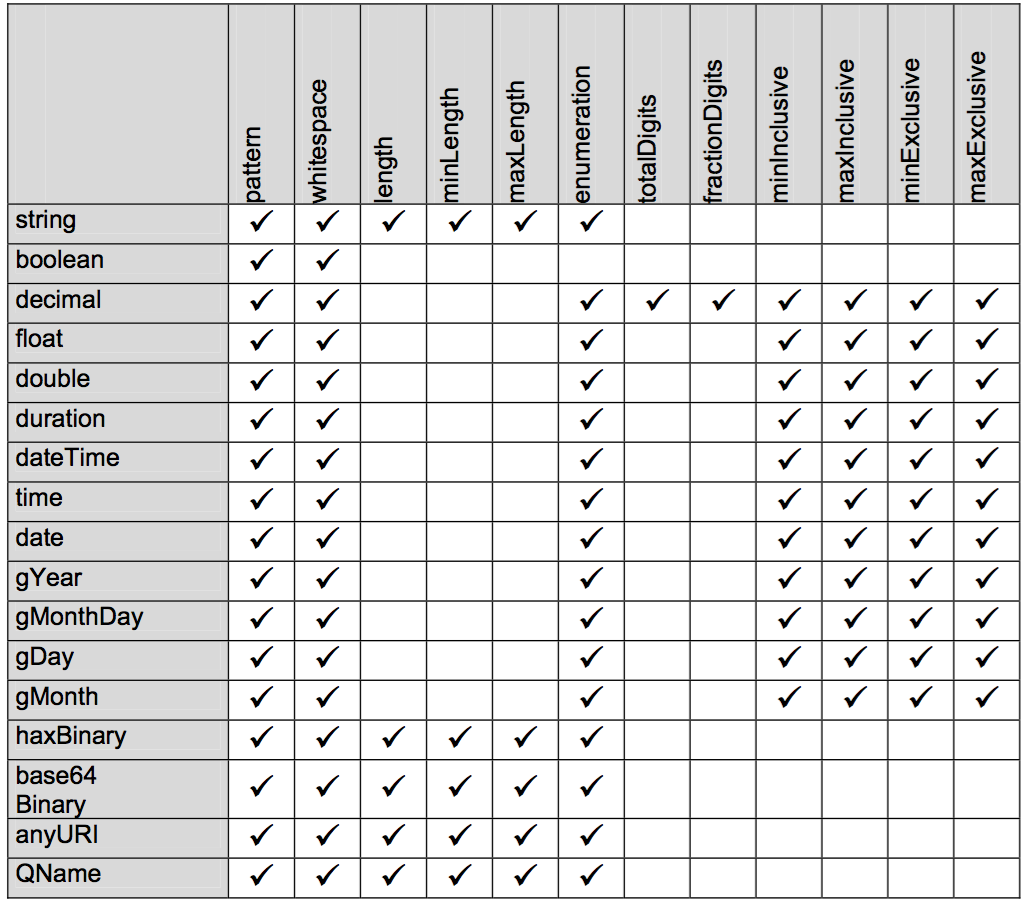
\includegraphics[width=.8\textwidth]{imgs/SchemaDataTypeFacets.png}
	\end{center}

\end{frame}



%Simple Type vs Complex Type

\begin{frame}
	\frametitle{Elementi per la definizione degli schemi xml}
	\framesubtitle{principi XSD}
	\addtocounter{nframe}{1}

	\begin{block}{Simple Type vs Complex Type}

		La differenza sostanziale tra un tipo semplice (\textit{simple types}) e un tipo complesso (\textit{complex types}) è che solo un tipo complesso può avere elementi figli e attributi.

	\end{block}

	\begin{block}{Simple Type vs Complex Type}

		Le entità \textit{simple type} possono trattare solo valori destrutturati. 
		\\Sia gli elementi sia gli attributi possono essere simple type.

	\end{block}

\end{frame}


% Simple types can only store a value. An element or attribute can have a simple type.
% Simple Types can be declared globally or locally. When a simple type is declared globally, it must always have a name.
% When a Simple Type is declared within the scope of an element or attribute it is a local declaration.
%% esempio (simpleTypeGlobalLocal)

\begin{frame}
	\frametitle{Elementi per la definizione degli schemi xml}
	\framesubtitle{principi XSD}
	\addtocounter{nframe}{1}

	\begin{center}
		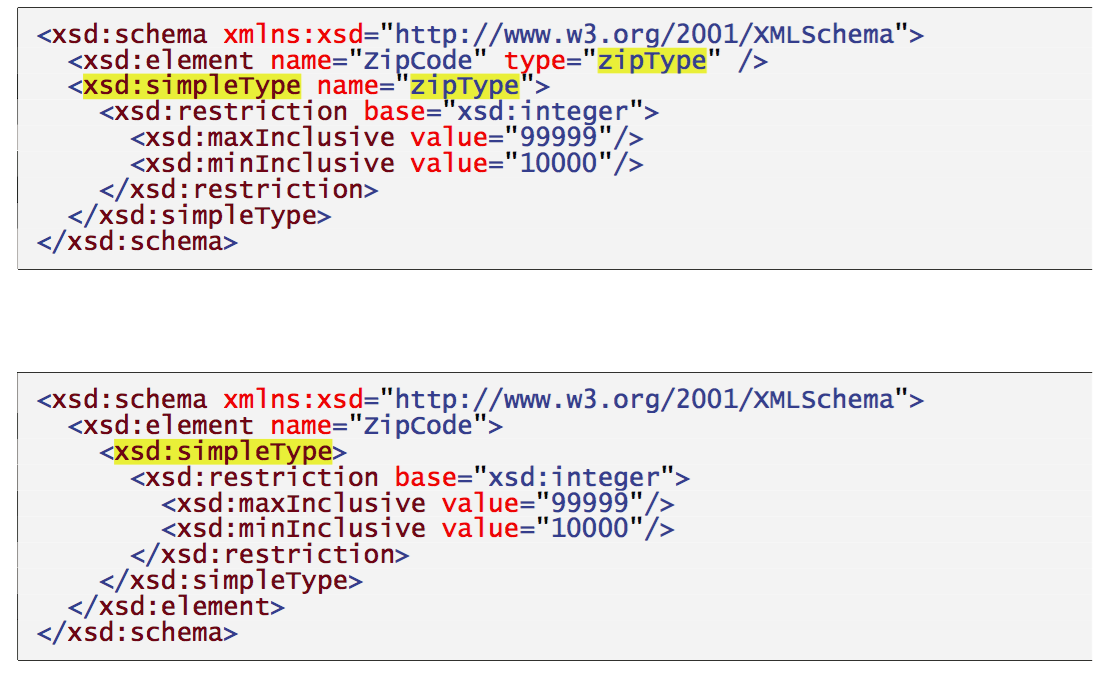
\includegraphics[width=.95\textwidth]{imgs/SimpleTypeGlobalLocal.png}
	\end{center}
	\textit{Simple Types can be declared \textbf{globally} or \textbf{locally}}

\end{frame}


\begin{frame}
	\frametitle{Elementi per la definizione degli schemi xml}
	\framesubtitle{principi XSD}
	\addtocounter{nframe}{1}

	\begin{block}{Global simple types}
		le definizioni di tipi globali sono utili per il riuso del codice e per mantenere ed organizzare al meglio una schema XSD ampio.
	\end{block}

	\textit{Molto utili quando bisogna uniformare un insieme di validazioni e manutenerle in modo coerente}

\end{frame}


\begin{frame}
	\frametitle{Elementi per la definizione degli schemi xml}
	\framesubtitle{principi XSD}
	\addtocounter{nframe}{1}

	\begin{block}{simple types: esercizio}
		\texttt{
			<xsd:simpleType name=``chapterNumberType''>
			<xsd:restriction base=``xsd:integer''>
			<xsd:maxInclusive value=``1000''/>
			<xsd:minInclusive value=``1''/>
			</xsd:restriction>
			</xsd:simpleType>
		}
	\end{block}

	\begin{block}{simple types: esercizio}
		\texttt{
			<xsd:element name=``item''>
			<xsd:complexType>
			<xsd:attribute name=``originalChapter'' type=``chapterNumberType''/>
			</xsd:complexType>
			</xsd:element>
		}
	\end{block}
\end{frame}


% Deriving

\begin{frame}
	\frametitle{Elementi per la definizione degli schemi xml}
	\framesubtitle{principi XSD}
	\addtocounter{nframe}{1}

	\begin{block}{simple types: deriving}
		Un nuovo tipo può essere derivato da un tipo già dichiarato (primitivo o meno) ed ereditarne le caratteristiche.
	\end{block}

	\begin{block}{simple types example}
		\begin{itemize}
			\item Derive by restriction
			\item Derive by list
			\item Derive by Union
		\end{itemize}
	\end{block}

\end{frame}

\begin{frame}
	\frametitle{Elementi per la definizione degli schemi xml}
	\framesubtitle{principi XSD}
	\addtocounter{nframe}{1}

	\begin{block}{simple types: deriving}
		Identificare il \textbf{tipo di dato di base} e aggiungere le dichiarazioni di \textbf{restrizione} e le \textbf{regole di validazione} che si reputano utili.
	\end{block}

\end{frame}

\begin{frame}
	\frametitle{Elementi per la definizione degli schemi xml}
	\framesubtitle{principi XSD}
	\addtocounter{nframe}{1}

	\begin{block}{simple types: deriving by Restriction}
		A restriction is defined by adding
		Un restrizione si definisce aggiungendo \textbf{``xsd:restriction''} alla dichiarazione del \textit{Simple Type}. 
	\end{block}

	\textbf{Ciascun tipo di dato possiede una collezione di proprietà (facets) attraverso le quali definire la restrizione voluta.}

\end{frame}

\begin{frame}
	\frametitle{Elementi per la definizione degli schemi xml}
	\framesubtitle{principi XSD}
	\addtocounter{nframe}{1}

	\begin{block}{simple types: deriving by Restriction}
		\texttt{
			<xsd:simpleType name=``signatureType''>
			\emph{<xsd:restriction base=``xsd:integer''>}
			\emph{<xsd:totalDigits value=``5''/>}
			</xsd:restriction>
			</xsd:simpleType>
		}
	\end{block}

	\begin{block}{simple types: deriving by Restriction}
		\texttt{
			<xsd:element name=``signature'' type=``signatureType''>
		}
		
		
		\texttt{
			<signature>12345</signature>
		} \textit{(valido)}
		\\\texttt{
			<signature>123ab</signature>
		} \textit{(non valido)}
	\end{block}
\end{frame}

% Another way of creating a new Simple Type is by deriving by List: 

\begin{frame}
	\frametitle{Elementi per la definizione degli schemi xml}
	\framesubtitle{principi XSD}
	\addtocounter{nframe}{1}

	\begin{block}{simple types: deriving by List}
		Un data type può contenere una lista di valori separata da spazi
	\end{block}

	\begin{block}{simple types: deriving by List}
		\texttt{<xsd:simpleType name=``chapterNumberList''>
			\emph{<xsd:list itemType=``xsd:integer'' />}
			</xsd:simpleType>}
		\\\texttt{
			<xsd:element name=``chapters'' type=``chapterNumberList'' />}
		\\\texttt{
			\textit{<chapters>1 53 60 61 205 409</chapters>}}
	\end{block}

\end{frame}

\begin{frame}
	\frametitle{Elementi per la definizione degli schemi xml}
	\framesubtitle{principi XSD}
	\addtocounter{nframe}{1}

	\begin{block}{simple types: deriving by Union}
		Un tipo derivato può accettare valori di qualsiasi tipo dichiarato nella derivazione.
	\end{block}

	\begin{block}{simple types: deriving by Union}
		\texttt{<xsd:simpleType name=``ZipCityUnion''>
			<xsd:union>
			<xsd:simpleType>
			<xsd:restriction base="ZipType"/>
			</xsd:simpleType>
			<xsd:simpleType>
			<xsd:restriction base="CityType"/>
			</xsd:simpleType>
			</xsd:union>
			</xsd:simpleType>}

	\end{block}

\end{frame}



% A third method of deriving a simple type is by union. The derived type can store the values acceptable to any of the base types from which the new type is derived.
% esempio:

% <xsd:simpleType name="ZipCityUnion">
%  <xsd:union>
%    <xsd:simpleType>
%      <xsd:restriction base="ZipType"/>
%    </xsd:simpleType>
%    <xsd:simpleType>
%      <xsd:restriction base="CityType"/>
%    </xsd:simpleType>
%  </xsd:union>
% </xsd:simpleType>

% The value will be accepted only if it validates successfully with one of the base types.

% It is not allowed to make the value space of a derived type less restrictive than the base type.

\begin{frame}
	\frametitle{Elementi per la definizione degli schemi xml}
	\framesubtitle{principi XSD}
	\addtocounter{nframe}{1}

	\begin{block}{simple types: deriving}
		I valori sono accettati solo se sono validi per uno dei tipi dichiarati nella derivazione.
	\end{block}

	\begin{block}{simple types: deriving}
		Nei costrutti di derivazione\textit{ non è permesso aumentare lo spazio dei valori consentiti}.
		\\\textbf{Non è possibile} quindi definire regole meno restrittive di quelle che caratterizzano il tipo di base.
	\end{block}
\end{frame}


% each XSD data type has a certain number of facets that control its value space.
% When we derive a new Simple Type from another, the new type will inherit all the facets of the base type. You can set the "fixed" attribute of the given facets to "true" to make sure that the derived types do not modify those facets.

\begin{frame}
	\frametitle{Elementi per la definizione degli schemi xml}
	\framesubtitle{principi XSD}
	\addtocounter{nframe}{1}

	\begin{block}{simple types: deriving facets}
		\textbf{Quando si deriva un tipo semplice da un altro tipo semplice, tutte le facets vengono ereditate.}
	\end{block}

	\begin{block}{simple types: deriving facets}
		
		E' possibile utilizzare l'attributo \textbf{fixed} di una data proprietà (facets) a \textbf{true} per assicurare che la proprietà stessa non venga modificata dal tipo derivato.
	\end{block}

\end{frame}


\begin{frame}
	\frametitle{Elementi per la definizione degli schemi xml}
	\framesubtitle{principi XSD}
	\addtocounter{nframe}{1}

	\begin{block}{Simple types: controllare la derivazione}
		XSD ha anche un meccanismo per controllare e proteggere (vietare) un tipo dall'essere derivato.
		\\ Si impiega l'attributo \textbf{final} della dichiarazione di simple type.
	\end{block}

\end{frame}

\begin{frame}
	\frametitle{Elementi per la definizione degli schemi xml}
	\framesubtitle{principi XSD}
	\addtocounter{nframe}{1}

	\begin{block}{controllare la derivazione: l'attributo final}
		\begin{itemize}
			\item restriction
			\item list
			\item union
			\item extension
			\item \#all
		\end{itemize}
	\end{block}

\end{frame}


\begin{frame}
	\frametitle{Elementi per la definizione degli schemi xml}
	\framesubtitle{principi XSD}
	\addtocounter{nframe}{1}

	\begin{block}{Simple types: controllare la derivazione - esempio}
		\texttt{
			<xsd:schema xmlns:xsd=``http://www.w3.org/2001/XMLSchema''>
			\emph{<xsd:simpleType name=``zipType'' final=``restriction union list extension''>}
			<xsd:restriction base=``xsd:integer''>
			\emph{<xsd:maxInclusive value=``99999'' fixed=``true''/>}
			<xsd:minInclusive value=``10000''/>
			</xsd:restriction>
			</xsd:simpleType>
			</xsd:schema>
		}
	\end{block}

\end{frame}

\begin{frame}
	\frametitle{Elementi per la definizione degli schemi xml}
	\framesubtitle{principi XSD}
	\addtocounter{nframe}{1}

	\begin{block}{Simple types: controllare la derivazione - esempio}
		Il termine estensione si riferisce alla possibilità di derivare un nuovo tipo che risulta essere complex type da un tipo base simple type.
	\end{block}

	\begin{block}{Simple types: controllare la derivazione - esempio}
		Quando l'attributo  \textbf{final} ha valore \textbf{\#all}, il Simple Type non puà essere derivato in alcun modo.
	\end{block}

\end{frame}


% Defining Enumerations
% Sometimes we will come across requirements where we need to apply a certain restriction to an element or attribute so that only a set of predefined values can be stored. 

% XSD Built-in Data Types: Primitive and Derived Data Types
% Facets of built-in data types
% XSD Built-in Derived data types
%% XSD has twenty-five such data types that derive directly or indirectly from one of the Primitive Data types
% xsd:integer is derived from xsd:decimal by restriction
% esempio

%<xs:simpleType name="integer" id="integer">
%  <xs:annotation>
%     <xs:documentation
%       source="http://www.w3.org/TR/xmlschema-2/#integer"/>
%   </xs:annotation>
%   <xs:restriction base="xs:decimal">
%     <xs:fractionDigits fixed="true" value="0"
%                        id="integer.fractionDigits"/>
%     <xs:pattern value="[\-+]?[0-9]+"/>
%   </xs:restriction>
%  </xs:simpleType>

% fractionDigits is a facet exposed by all numeric data types and it restricts the number of decimal places in the value. 
% The attribute fixed indicates that any type that derives from integer is not allowed to modify the value of fractionDigits facet.
% It applies a pattern restriction to validate the format of the value.
% as with integer, each of the XSD built-in derived data types derives from one of the Primitive Types directly or indirectly.

% Facets of Data Types
%% Each data type has a certain set of characteristics that can be used to perform additional validations on the value. Each of the XSD data types has a certain number of such properties that add additional restrictions on the value. These properties are called facets in XSD. Not all data types support the same facets.

% list of all the facets supported by the different data types of XSD.
% length restricts the number of characters a value can accept.
% minLength defines the minimum length of the value
% maxLength defines the maximum length of the value
% pattern specifies a Regular Expression to validate the value.
% enumeration is used to restrict the values to a set of predefined choices
% whitespace defines the way whitespaces is processed by the schema processor (Preserve, replace, collapse).
% totalDigits restricts the number of digits the type can hold (cifre intere + decimali)
% fractionDigits restricts the number of digits in the decimal part of the value
% maxInclusive specifies the highest value the type can accept
% minInclusive specifies the highest numeric value the type can accept, excluding the value specified in the restriction.
% maxExclusive defines the lowest value that the type can accept.
% minExclusive defines the minimum value that the type can accept, excluding the value specified in the restriction

%% foto della tabella (schemaDatatypeFacets)

%% Tipi di dati xsd derivati da tipi di dati primitivi (25 in totale)
%% immagini per i tipi e esempi di catena di derivazione (DerivedTypeBaseType, DerivedTypeFromDerivedType, NumericalDerivedType, NumericalGrafico, String-Grafico).

% complex type
\begin{frame}
	\frametitle{Elementi per la definizione degli schemi xml}
	\framesubtitle{principi XSD}
	\addtocounter{nframe}{1}

	\begin{block}{Complex Type}
		Un tipo coomplesso (\textbf{complex type}) può essere strutturato e quindi avere figli e avere attributi.
		% an element has a Simple Type, it cannot have child elements or attributes. It can store only a text value.

	\end{block}

	\begin{block}{Named Complex types}
		Una comples type può avere un nome (\textit{Named Complex Type}) così da poter essere impiegato all'interno della dichiarazione di altri tipi complessi.
	\end{block}

	\textbf{le Attribute declarations non possono avere Complex Types.}

\end{frame}



%% Esempio:

\begin{frame}
	\frametitle{Elementi per la definizione degli schemi xml}
	\framesubtitle{principi XSD}
	\addtocounter{nframe}{1}

	\begin{block}{Named Complex Type Esempio}
		\texttt{
			<xsd:complexType name=``addressType''>
			<xsd:all>
			<xsd:element name="address"/>
			<xsd:element name="street"/>
			<xsd:element name="settlment"/>
			<xsd:element name="country"/>
			</xsd:all>
			</xsd:complexType>
		}
	\end{block}

\end{frame}

\begin{frame}
	\frametitle{Elementi per la definizione degli schemi xml}
	\framesubtitle{principi XSD}
	\addtocounter{nframe}{1}

	\begin{block}{Named Complex types Esempio}
		\texttt{
			<xsd:element name=``AddressDivision''>
			<xsd:complexType>
			<xsd:sequence>
			<xsd:element name="addressee"/>
			<xsd:element name="address" type="addressType"/>
			</xsd:sequence>
			</xsd:complexType>
			</xsd:element>
		}
	\end{block}

\end{frame}

\begin{frame}
	\frametitle{Elementi per la definizione degli schemi xml}
	\framesubtitle{principi XSD}
	\addtocounter{nframe}{1}

	\begin{block}{Complex Type}
		I 
		Named Complex Types offrono un potente strumento per riusare parti di codifica XSD all'interno dello schema.
		\\ Mentre Anonymous Complex Types nono possono essere riferiti e appaiono solo all'interno della dichiarazione in cui vengono definiti.

	\end{block}

	\begin{block}{Anonymous Complex types}
		\texttt{
			<xsd:element name=``Customer''>
			<xsd:complexType>
			<xsd:sequence>
		}
	\end{block}
\end{frame}

%% esempio
% <xsd:schema xmlns:xsd="http://www.w3.org/2001/XMLSchema">
%   <!-- Customer Information -->
%   <xsd:element name="Customer">
%     <xsd:complexType>
%       <xsd:sequence>
%         <xsd:element name="CustomerName"/>
%         <xsd:element name="Address">
%           <xsd:complexType>
%             <xsd:all>
%               <xsd:element name="Address"/>
%               <xsd:element name="Street"/>
%               <xsd:element name="City"/>
%               <xsd:element name="Zip"/>
%               <xsd:element name="State"/>
%             </xsd:all>
%           </xsd:complexType>
%         </xsd:element>
%       </xsd:sequence>
%     </xsd:complexType>
%   </xsd:element>
% </xsd:schema>

\begin{frame}
	\frametitle{Elementi per la definizione degli schemi xml}
	\framesubtitle{principi XSD}
	\addtocounter{nframe}{1}

	\begin{block}{Content Model}
		\textbf{La struttura di un Complex Type è chiamata Content Model.}
	\end{block}

	\begin{block}{Content Model: Simple Content, Complex Content}
		\begin{itemize}
			\item \textbf{Simple Content}: contiene valori testuali e può avere attributi.
			\item \textbf{Complex Content}: \textit{empty}, \textit{element- only }, \textit{mixed type}.
		\end{itemize}
	\end{block}
\end{frame}

\begin{frame}
	\frametitle{Elementi per la definizione degli schemi xml}
	\framesubtitle{principi XSD}
	\addtocounter{nframe}{1}

	\begin{block}{Content Model: complex content}
		\begin{itemize}
			\item \textit{Empty} content può avere attributi.
			\item \textit{element-only} ha elementi figli, può avere attributi, ma non può avere testo come valore dell'elemento.
			\item \textit{mixed content} può contenere elementi figli, attributi e valori testuali.
		\end{itemize}
	\end{block}
\end{frame}


% Esempio mexed content:
% <Email Priority="High">
%   Dear <name>Jacob</name>,
%   Your order has been
%   shipped on <date>2008-01-01</date>
% </Email>

%% Simple Content
% when an element has Simple Content it can store a text value and can have attributes.
% Simple Content does not allow child elements

%% Esempio:
%<xsd:schema xmlns:xsd="http://www.w3.org/2001/XMLSchema">
%  <xsd:element name="Phone">
%     <xsd:complexType>
%       <xsd:simpleContent>
%         <xsd:extension base="xsd:string">
%           <xsd:attribute name="location" type="xsd:string"/>
%         </xsd:extension>
%       </xsd:simpleContent>
%     </xsd:complexType>
%   </xsd:element>
% </xsd:schema>

\begin{frame}
	\frametitle{Elementi per la definizione degli schemi xml}
	\framesubtitle{principi XSD}
	\addtocounter{nframe}{1}

	\begin{block}{Complex type: Simple Content}
		\textit{Simple Content}: text value e attributi, ma non puà avere figli.
	\end{block}

	\begin{block}{Complex type: Simple Content esempio}
		\texttt{
			<xsd:element name=``name''>
			\emph{<xsd:complexType>}
			\emph{<xsd:simpleContent>}
			<xsd:extension base=``xsd:string''>
			\emph{<xsd:attribute name="type" type="xsd:string"/>}
			</xsd:extension>
			</xsd:simpleContent>
			</xsd:complexType>
			</xsd:element>
		}
	\end{block}
\end{frame}


\begin{frame}
	\frametitle{Elementi per la definizione degli schemi xml}
	\framesubtitle{principi XSD}
	\addtocounter{nframe}{1}

	\begin{block}{Complex type: Complex Content - Empty content}
		Gli elementi Complex Type che hanno un modello del contenuto complesso vuoto sono simili agli elementi di tipo complesso con contenuto semplice.
	\end{block}

	\begin{block}{Complex type: Empty content}
		Gli elementi Empty content compex types non possono contenere testo, ma possono avere attributi.
	\end{block}
\end{frame}


%% Empty content
% Complex Types having empty content are very close to the ones having simple content, but they cannot store a text value. However, it can have attributes.

\begin{frame}
	\frametitle{Elementi per la definizione degli schemi xml}
	\framesubtitle{principi XSD}
	\addtocounter{nframe}{1}

	\begin{block}{Complex type: element-only content}
		Gli elementi  Complex Types element-only content hanno un modello del contenuto composto solo da elementi figli e attributi, ma non possono contenere del testo.
	\end{block}
\end{frame}

\begin{frame}
	\frametitle{Elementi per la definizione degli schemi xml}
	\framesubtitle{principi XSD}
	\addtocounter{nframe}{1}

	\begin{block}{Complex type: element-only content - esempio}
		\texttt{
			\emph{<xsd:group name=``fileDesc''>}
			<xsd:sequence>
			<xsd:element name="titleStmt"/>
			<xsd:element name="publicationStmt"/>
			<xsd:element name="sourceDesc" />
			</xsd:sequence>
			</xsd:group>
			<xsd:element name=``teiHeader''>
			\emph{<xsd:complexType>}
			<xsd:sequence>
			\emph{<xsd:group ref=``fileDesc''/>}
			</xsd:sequence>
			</xsd:complexType>
			</xsd:element>
			</xsd:schema>
		}
	\end{block}
\end{frame}

%% Mixed Content
\begin{frame}
	\frametitle{Elementi per la definizione degli schemi xml}
	\framesubtitle{principi XSD}
	\addtocounter{nframe}{1}

	\begin{block}{Complex type: mixed content}
		Gli elementi Mixed Content hanno un modello del contenuto che combina il simple content e l'element-only content.
		\\ \textbf{Può contenere elementi figli, testo e attributi.}
	\end{block}

	\begin{block}{Complex type: mixed content}
		Un parser XML può estrarre molte più informazioni se un elemento ha un modello del contenuto The Mixed content.
	\end{block}
\end{frame}

\begin{frame}
	\frametitle{Elementi per la definizione degli schemi xml}
	\framesubtitle{principi XSD}
	\addtocounter{nframe}{1}

	\begin{block}{Complex type: mixed content - esempio}
		\texttt{
			<xsd:element name=``seg''>
			<xsd:complexType \textit{mixed=``true''}>
			<xsd:all>
			<xsd:element name="name"/>
			<xsd:element name="quote"/>
			</xsd:all>
			</xsd:complexType>
			</xsd:element>
			</xsd:schema>
		}
	\end{block}

	\begin{block}{Complex type: mixed content - esempio}
		\texttt{
			<seg><name>Petrarca</name> disse: <quote>Raramente la grande bellezza e la grande virtù dimorano assieme</quote></seg>
		}
	\end{block}

\end{frame}

\begin{frame}
	\frametitle{Elementi per la definizione degli schemi xml}
	\framesubtitle{principi XSD}
	\addtocounter{nframe}{1}

	\begin{block}{Complex type: mixed content}
		\textit{La sola differenza con il modello di contenuto element-only è la presenza dell'attributo ``\textbf{mixed}.'' Nel campo delle Digital Scholarly Editions ci sono moltissimi casi in cui utilizziamo questo tipo di contenuto misto}
	\end{block}


\end{frame}


\begin{frame}
	\frametitle{Elementi per la definizione degli schemi xml}
	\framesubtitle{principi XSD}
	\addtocounter{nframe}{1}

	\begin{block}{Complex type con attributi}
		Se un elementoo di tipo complesso contiene dichiarazioni di elementi e di attributi, la dichiarazione degli attributi \textbf{segue} la dichiarazione degli elementi.
	\end{block}

	\begin{block}{Complex type: mixed content}
		\texttt{<xsd:element name=``seg''>
			<xsd:complexType \textit{mixed=``true''}>
			<xsd:sequence>
				\emph{<xsd:element name="quote"/>}
			</xsd:sequence>
			\emph{<xsd:attribute name="part"/>}
			</xsd:complexType>
			</xsd:element>
			</xsd:schema>}
	\end{block}
\end{frame}

\begin{frame}
	\frametitle{Elementi per la definizione degli schemi xml}
	\framesubtitle{principi XSD}
	\addtocounter{nframe}{1}

	\begin{block}{Elementi e Attributi: ordering}
		Gli attributi di un elemento possono apparire in qualsiasi ordine.
		\\\textit{La posizione (ordine) di apparizione non è significativa.}

	\end{block}

	\begin{block}{Elementi e Attributi: ordering}
		\textit{La posizione (ordine) degli elementi all'interno di un documento XML è significativa.}
		Quindi è importante avere un meccanismo per specificare la \textbf{politica di ordinamento} all'interno del content model di un elemento.
	\end{block}
\end{frame}


\begin{frame}
	\frametitle{Elementi per la definizione degli schemi xml}
	\framesubtitle{principi XSD}
	\addtocounter{nframe}{1}

	\begin{block}{Elementi e Attributi: ordering}
		\begin{itemize}
			\item \textbf{sequence}: è un elemento (\texttt{<xsd:sequence />}) che indica che gli elementi dichiarati devono seguire esattamente l'ordine specificato.
			\item \textbf{all}: è un elemento (\texttt{<xsd:all>}) che indica che l'ordine degli elementi non è significativo.
			\item \textbf{choice}: è un elemento (\texttt{<xsd:choice />}) che indica che solo uno dell'insieme di elementi specificato può essere usato nel documento XML.
		\end{itemize}
	\end{block}
\end{frame}

\begin{frame}
	\frametitle{Elementi per la definizione degli schemi xml}
	\framesubtitle{principi XSD}
	\addtocounter{nframe}{1}

	\begin{block}{Elementi e Attributi: occurrence indicator}
		Gli attributi non possono apparire più di una volta all'interno dell'elemento.
	\end{block}

	\begin{block}{Elementi e Attributi: occurrence indicator}
		Un Elemento può apparire più di una volta all'interno del proprio elemento padre/contenitore.
		\\Possiamo controllare quante occorrenze di un elemento sono consentite grazie agli attributi \textbf{minOccurs} e \textbf{maxOccurs}
	\end{block}
\end{frame}


\begin{frame}
	\frametitle{Elementi per la definizione degli schemi xml}
	\framesubtitle{principi XSD}
	\addtocounter{nframe}{1}


	% esempio: The following table shows a few examples that demonstrate how to control the occurrences of elements by using minOccurs and maxOccurs. % (immagine:TabellaMinMaxOccurs).

	\begin{center}
		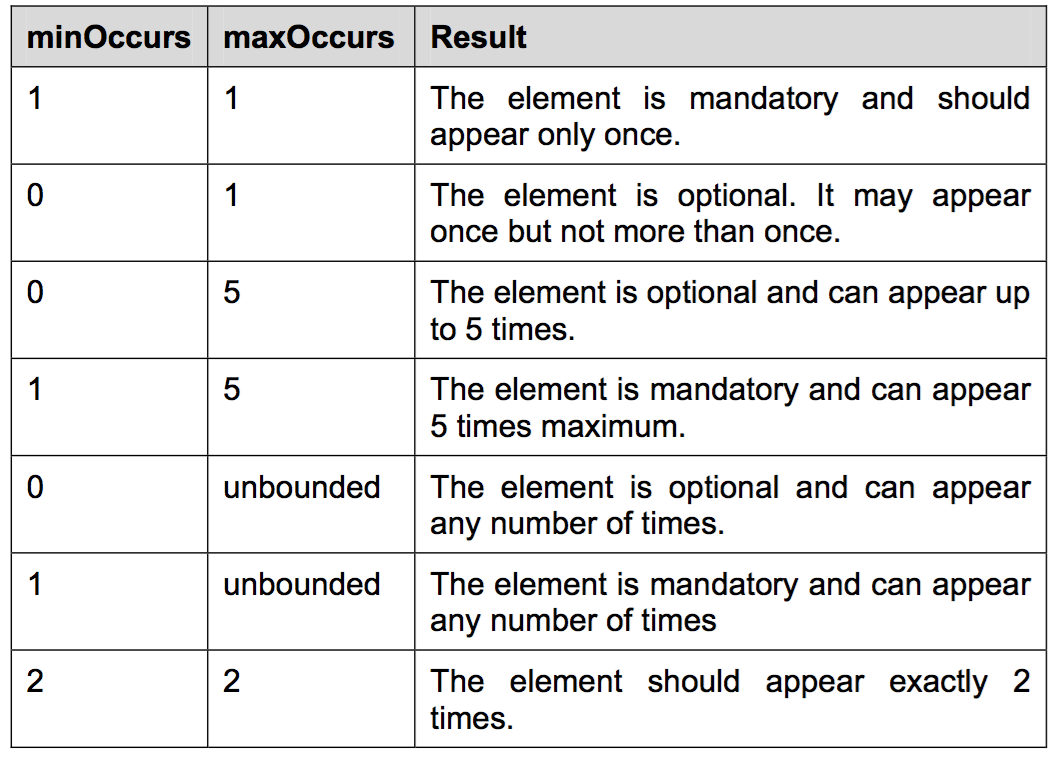
\includegraphics[width=.95\textwidth]{imgs/tabellaMinMaxOccurs.png}
	\end{center}

\end{frame}


%% Element Groups
% provide reusability to a certain extent as they can be inserted into other complex types within the same schema. The schema is easier to modify and maintain.
%% esemipio:
%<xsd:schema xmlns:xsd="http://www.w3.org/2001/XMLSchema">
%   <xsd:group name="ContactInfo">
%     <xsd:sequence>
%       <xsd:element name="email"/>
%       <xsd:element name="phone"/>
%     </xsd:sequence>
%   </xsd:group>
%   <xsd:element name="author">
%     <xsd:complexType>
%       <xsd:sequence>
%         <xsd:group ref="ContactInfo"/>
%       </xsd:sequence>
%    </xsd:complexType>
%   </xsd:element>
% </xsd:schema>
% Una possibile istanza di documento XML validata dallo schema di cui sopra:
% <author>
%       <email>name@institution.it</email>
%       <phone>0039123456789</phone>
% </author>



% Complex type derivation

\begin{frame}
	\frametitle{Elementi per la definizione degli schemi xml}
	\framesubtitle{principi XSD}
	\addtocounter{nframe}{1}

	\begin{block}{Content Model: Deriving}
		Nuovi tipi complessi possono essere derivati da tipi complessi con modello del contentuo Simple Content.
		\textit{Non è possibile derivare Compex Content da Simple Content.}
	\end{block}

	\begin{block}{Content Model: Complex Content}
		Un elemento con modello Complex Content può contenere elementi figli, attributi e testo.
	\end{block}
\end{frame}

% Complex Type derivation
\begin{frame}
	\frametitle{Elementi per la definizione degli schemi xml}
	\framesubtitle{principi XSD}
	\addtocounter{nframe}{1}

	\begin{block}{Content Model: Complex Content}
		\textbf{Nuovi complex types possono essere derivati da complex type già definiti \textit{by restriction} oppure \textit{by extension}}
	\end{block}
\end{frame}

\begin{frame}
	\frametitle{Elementi per la definizione degli schemi xml}
	\framesubtitle{principi XSD}
	\addtocounter{nframe}{1}

	\begin{block}{Complex Type derivation: da simple type}
		E' possibile derivare complex type da un tipo base simple type, ma solo se l'elemento è simple content.
		\\Se l'attributo \textit{final} è impostato sul valore \textbf{extension}, il tipo base (simple type) non può essere esteso.

	\end{block}

\end{frame}

\begin{frame}
	\frametitle{Elementi per la definizione degli schemi xml}
	\framesubtitle{principi XSD}
	\addtocounter{nframe}{1}

	\begin{block}{Complex Type derivation: da simple type - esempio}
		\texttt{
			<xsd:complexType name=``divTypeEx''>
			\emph{<xsd:simpleContent>}
			\emph{<xsd:extension base=``divType''>}
			\emph{<xsd:attribute name=``type'' use=``required''/>}
			</xsd:extension>
			</xsd:simpleContent>
			</xsd:complexType>
		}
	\end{block}
\end{frame}

\begin{frame}
	\frametitle{Elementi per la definizione degli schemi xml}
	\framesubtitle{principi XSD}
	\addtocounter{nframe}{1}

	\begin{block}{Complex Type derivation: Diversi casi}
		\begin{itemize}
			\item derivare un nuovo tipo by restriction oppure by extension da un complex type simple content model
			\item derivare by restriction da un complex type con simple content
			\item aggiungere restrizioni al content/text di un elemento
			\item aggiungere restrizioni ad un attributo
			\item eleminare uno o più attributi ad un tipo di elemento
		\end{itemize}
	\end{block}
	\textit{Le politiche di derivazione cambiano a seconda del modello di contenuto del tipo considerato}

\end{frame}

%% Esempio:
\begin{frame}
	\frametitle{Elementi per la definizione degli schemi xml}
	\framesubtitle{principi XSD}
	\addtocounter{nframe}{1}

	\begin{block}{Complex Type derivation: esempio}
		\texttt{
		<xsd:complexType name=``RestrictedPhoneType''>
		\emph{<xsd:simpleContent>}
		\emph{<xsd:restriction base=``PhoneType''>}
		<xsd:pattern value="[0-9]{3}-[0-9]{3}-[0-9]{4}"/>
		\emph{<xsd:attribute name=``Type''>}
		\emph{<xsd:simpleType>}
		<xsd:restriction base=``xsd:string''>
		<xsd:enumeration value="Home"/>
		<xsd:enumeration value="Work"/>
		</xsd:restriction>
		</xsd:simpleType>
		</xsd:attribute>
		\emph{<xsd:attribute name="CallOnWeekend" type="xsd:boolean" use="prohibited"/> }
		</xsd:restriction>
		</xsd:simpleContent>
		</xsd:complexType>
		}
	\end{block}
\end{frame}


\begin{frame}
	\frametitle{Elementi per la definizione degli schemi xml}
	\framesubtitle{principi XSD}
	\addtocounter{nframe}{1}

	\begin{block}{Complex Type derivation}
		Si noti l'attributo \textbf{use} con valore \textit{prohibited}.
		\\ Se si vuole eliminare un attributo è necessario ridefinirlo nel tipo derivato e impostare l'attributo \textit{use} al valore \textit{prohibited}.
	\end{block}

	\begin{block}{Complex Type derivation}
		Se un attributo è obbligatorio \textit{required} nel tipo base, non è possibile cambiarlo in \textit{optional} nel tipo derivato (non è possibile avere un tipo derivato meno restrittivo del tipo base).
	\end{block}
\end{frame}

\begin{frame}
	\frametitle{Elementi per la definizione degli schemi xml}
	\framesubtitle{principi XSD}
	\addtocounter{nframe}{1}

	\begin{block}{Complex Type derivation}
		\textbf{ Quando si deriva by extension da un tipo complesso con simple content, il tipo risultante sarà sempre un simple content.}
	\end{block}

	\textit{L'unca cosa che è possibile fare è aggiungere attributi}

\end{frame}


\begin{frame}
	\frametitle{Elementi per la definizione degli schemi xml}
	\framesubtitle{principi XSD}
	\addtocounter{nframe}{1}

	\begin{block}{Complex Type derivation: simple content esempio}
		\texttt{
			<xsd:complexType name=``ExtendedPhoneType''>
			\emph{<xsd:simpleContent>}
			\emph{<xsd:extension base=``PhoneType''>}
				<xsd:attribute name="CallOnHolidays" type="xsd:string"/>
			</xsd:extension>
			</xsd:simpleContent>
			</xsd:complexType>
		}
	\end{block}


\end{frame}

%% esempio:
% <xsd:complexType name="ExtendedPhoneType">
%   <xsd:simpleContent>
%     <xsd:extension base="PhoneType">
%       <xsd:attribute name="CallOnHolidays" type="xsd:string"/>
%     </xsd:extension>
%   </xsd:simpleContent>
% </xsd:complexType>


\begin{frame}
	\frametitle{Elementi per la definizione degli schemi xml}
	\framesubtitle{principi XSD}
	\addtocounter{nframe}{1}

	\begin{block}{Complex Type derivation}
		Un tipo complesso \textit{element-only content} può essere esteso (extended) o limitato (restricted) per generare un nuovo tipo.
	\end{block}

	\begin{block}{Complex Type derivation}
		Derivare \textit{by restriction} da un tipo \textit{element-only content} vuol dire eliminare elementi o attributi.
		\\\textbf{Attenzione: gli elementi del tipo di base non vengono passati al tipo derivato (a differenza degli attributi)}
	\end{block}
\end{frame}


\begin{frame}
	\frametitle{Elementi per la definizione degli schemi xml}
	\framesubtitle{principi XSD}
	\addtocounter{nframe}{1}

		%\textbf{Tutti gli elementi obbligatori nel tipo di base devono essere presenti anche nel tipo derivato}
	
	\begin{block}{Complex Type derivation}
		\begin{itemize}
			\item Se gli elementi nel tipo di base sono dichiarati all'interno di una \textit{sequence}, il tipo derivato non può cambiare tale dichiarazione in \textit{all} oppure \textit{choice}.
			\item Se il tipo di base ha specificato gli elementi con una dichiarazione \textit{all}, il tipo derivato può cambiare la dichiarazione con \textit{sequence}. 
			\item Se il tipo di base ha specificato gli elementi con la dichiarazione \textit{choice}, il tipo derivato deve avere ugualmente la dichiarazione \textit{choice}.
		\end{itemize}
	\end{block}
\end{frame}

\begin{frame}
	\frametitle{Elementi per la definizione degli schemi xml}
	\framesubtitle{principi XSD}
	\addtocounter{nframe}{1}

	
	\begin{block}{Complex Type derivation}
		\begin{itemize}
			\item Se si vuole rimuovere un attributo bisogna dichiararlo nuovamente e specificarne l'uso \textit{prohibited}.
			\item Un tipo derivato non può eliminare un attributo dichiarato obbligatorio nel tipo di base.
			\item Bisogna ridefinire un attributo nel tipo derivato, solo se si vuole limitare il suo spazio di valori (\textit{gli attributi vengono ereditati dal tipo derivato}).
		\end{itemize}
	\end{block}
\end{frame}


% Esempio:

\begin{frame}
	\frametitle{Elementi per la definizione degli schemi xml}
	\framesubtitle{principi XSD}
	\addtocounter{nframe}{1}

	\begin{block}{Complex Type derivation: esempio}
		%   <!-- Contact Element -->
		\texttt{\emph{<xsd:element name="Contact" type="RestrictedContactType"/>}}
		\\\texttt{%<!-- Contact Type -->
			<xsd:complexType name=``ContactType''>
			<xsd:sequence>
			<xsd:element name="Phone" minOccurs="0"/>
			<xsd:element name="Email" minOccurs="0"/>
			</xsd:sequence>
			<xsd:attribute name="Name" />
			<xsd:attribute name="Title"/>
			</xsd:complexType>}
	\end{block}
\end{frame}

\begin{frame}
	\frametitle{Elementi per la definizione degli schemi xml}
	\framesubtitle{principi XSD}
	\addtocounter{nframe}{1}

	\begin{block}{Complex Type derivation: esempio}
		%<!-- Restricted Contact Type -->
		\texttt{<xsd:complexType name=``RestrictedContactType''>
		\emph{<xsd:complexContent>}
		\emph{<xsd:restriction base=``ContactType''>}
		<xsd:sequence>
		<xsd:element name=``Phone''>
		<xsd:simpleType>
		<xsd:restriction base=``xsd:string''>
		<xsd:pattern value="[0-9]{3}-[0-9]{3}-[0-9]{4}"/>
		</xsd:restriction>
		</xsd:simpleType>
		</xsd:element>
		</xsd:sequence>
		\emph{<xsd:attribute name="Title" use="prohibited"/>}
		\emph{<xsd:attribute name=``Name'' type=``xsd:string''>}
		</xsd:attribute>
		</xsd:restriction>
		</xsd:complexContent>
		</xsd:complexType>}
	\end{block}
\end{frame}


\begin{frame}
	\frametitle{Elementi per la definizione degli schemi xml}
	\framesubtitle{principi XSD}
	\addtocounter{nframe}{1}

	\begin{block}{Complex Type derivation}
		E' possibile derivare un \textit{empty content} da un\textit{ element-only content}. 
		\\Ciò viene fatto mantenendo la \textit{dichiarazione di restrizione vuota}. 
		\\Questo \textbf{non vale per gli attributi}, che si ereditano tutti.
	\end{block}

	\begin{block}{Complex Type derivation}
		\textbf{Gli elementi del tipo dell'elemento base devono essere opzionali}
	\end{block}
\end{frame}


\begin{frame}
	\frametitle{Elementi per la definizione degli schemi xml}
	\framesubtitle{principi XSD}
	\addtocounter{nframe}{1}

	\begin{block}{Complex Type extension}
		\textit{I tipi \textbf{complex type} vengono estesi per aggiungere elementi e attributi}
	\end{block}

	\begin{block}{Complex Type extension}
		\textbf{Quando si deriva per estensione, sia tutti gli elementi, sia tutti gli attributi si ereditano dal tipo base al tipo derivato}.
	\end{block}
\end{frame}


% <xsd:schema xmlns:xsd="http://www.w3.org/2001/XMLSchema">
%   <!-- Contact Element -->
%   <xsd:element name="Contact" type="ExtendedContactType"/>
%   
%   <!-- Extended Contact Type -->
%   <xsd:complexType name="ExtendedContactType">
%     <xsd:complexContent>
%       <xsd:extension base="ContactType">
%         <xsd:sequence>
%           <xsd:element name="Fax"/>
%         </xsd:sequence>
%         <xsd:attribute name="Department"/>
%       </xsd:extension>
%     </xsd:complexContent>
%   </xsd:complexType>
%  
%    <!-- Contact Type -->
%   <xsd:complexType name="ContactType">
%     <xsd:sequence>
%       <xsd:element name="Phone"/>
%       <xsd:element name="Email" minOccurs="0"/>
%     </xsd:sequence>
%     <xsd:attribute name="Name" use="required"/>
%     <xsd:attribute name="Title"/>
%   </xsd:complexType>
% </xsd:schema>
%
%% Una possibile istanza XML:
% <Contact Name="Jacob" Title="Manager" Department="IT">
%   <Phone>999-888-7777</Phone>
%   <Email>jacob@jacob.com</Email>
%   <Fax>888-999-3333</Fax>
% </Contact>

\begin{frame}
	\frametitle{Elementi per la definizione degli schemi xml}
	\framesubtitle{principi XSD}
	\addtocounter{nframe}{1}

	\begin{block}{Complex Type derivation: esempio}
		%   <!-- Contact Element -->
		\texttt{\emph{<xsd:element name="Contact" type="ExtendedContactType"/>}}
		\texttt{%<!-- Contact Type -->
			<xsd:complexType name=``ContactType''>
			<xsd:sequence>
			<xsd:element name=``Phone''/>
			<xsd:element name=``Email'' minOccurs=``0''/>
			</xsd:sequence>
			<xsd:attribute name=``Name'' use=``required''/>
			<xsd:attribute name=``Title''/>
			</xsd:complexType>
			</xsd:schema>
		}
	\end{block}
\end{frame}


\begin{frame}
	\frametitle{Elementi per la definizione degli schemi xml}
	\framesubtitle{principi XSD}
	\addtocounter{nframe}{1}

	\begin{block}{Complex Type derivation: esempio}
		%<!-- Extended Contact Type -->
		\texttt{
			<xsd:complexType name=``ExtendedContactType''>
			\emph{<xsd:complexContent>}
			\emph{<xsd:extension base=``ContactType''>}
			<xsd:sequence>
			\emph{<xsd:element name=``Fax''/>}
			</xsd:sequence>
			\emph{<xsd:attribute name=``Department''/>}
			</xsd:extension>
			</xsd:complexContent>
			</xsd:complexType>
		}
	\end{block}
\end{frame}

\begin{frame}
	\frametitle{Elementi per la definizione degli schemi xml}
	\framesubtitle{principi XSD}
	\addtocounter{nframe}{1}

	\begin{block}{Complex Type: deriving }
		Si può derivare un \textit{mixed content} sia by restriction sia by extension.
		Derivare un tipo complesso \textit{mixed content} è simile a derivare un tipo complesso \textit{element-only}.
	\end{block}

	\begin{block}{Complex Type: deriving}
		 deriving by restriction un mixed content type: \textit{a mixed type}, \textit{element-only} oppure \textit{empty content}. 
	\end{block}
	\textit{Gli elementi dichiarati nel tipo base non si ereditano, gli attributi si ereditano}
\end{frame}


% esempio:
\begin{frame}
	\frametitle{Elementi per la definizione degli schemi xml}
	\framesubtitle{principi XSD}
	\addtocounter{nframe}{1}

	\begin{block}{Complex Type derivation: esempio}
		%<!-- Extended Contact Type -->
		\texttt{
			\emph{<xsd:complexType name="RestrictedNoteType" mixed=``true''>}
			\emph{<xsd:complexContent>}
			\emph{<xsd:restriction base=``NoteType''>}
			<xsd:sequence>
			<xsd:element name="name"/>
			</xsd:sequence>
			</xsd:restriction>
			</xsd:complexContent>
			</xsd:complexType>
		}
	\end{block}
	\textit{Rimuovendo l'attributo ``mixed'' dalla dichiarazione del tipo complesso si ottiene un element-only complex type da un tipo mixed content}
\end{frame}

\begin{frame}
	\frametitle{Elementi per la definizione degli schemi xml}
	\framesubtitle{principi XSD}
	\addtocounter{nframe}{1}
	\begin{block}{Complex Type: deriving - Mixed Content}
		Quando si deriva by restriction un mixed type, si può creare un \textit{empty content type} se tutti gli elementi del tipo base sono optionali. 
	\end{block}
	\begin{block}{Complex Type: deriving - Mixed Content}
		Per eliminare gli attributi c'è bisogno di dichiararli nel tipo derivato e di proibirne l'uso (\textit{prohibited attribute}).
	\end{block}
\end{frame}

% esempio
\begin{frame}
	\frametitle{Elementi per la definizione degli schemi xml}
	\framesubtitle{principi XSD}
	\addtocounter{nframe}{1}

	\begin{block}{Complex Type derivation: esempio}
		\texttt{
			\emph{<xsd:complexType name=``SimpleNoteType''>}
			\emph{<xsd:simpleContent>}
			<xsd:restriction base=``NoteType''>
			<xsd:simpleType>
			\emph{<xsd:restriction base="xsd:string"/>}
			</xsd:simpleType>
			</xsd:restriction>
			</xsd:simpleContent>
			</xsd:complexType>
		}
	\end{block}
	\textit{Le specifiche XSD permettono di derivare un simple content da un mixed-content type}
\end{frame}

% esempio
\begin{frame}
	\frametitle{Elementi per la definizione degli schemi xml}
	\framesubtitle{principi XSD}
	\addtocounter{nframe}{1}

	\begin{block}{Complex Type derivation: esempio}
		%   <!-- Note Type -->
		\texttt{
			<xsd:complexType name=``NoteType'' mixed=``true''>
			<xsd:sequence>
			<xsd:element name="name"/>
			<xsd:element name="mobile"/>
			</xsd:sequence>
			</xsd:complexType>
		}
	\end{block}
	\textit{Quando si deriva by \textbf{extension}, possiamo solo generare \textbf{mixed content complex type}}
\end{frame}


\begin{frame}
	\frametitle{Elementi per la definizione degli schemi xml}
	\framesubtitle{principi XSD}
	\addtocounter{nframe}{1}

	\begin{block}{Complex Type derivation: esempio}
		\texttt{\emph{<xsd:element name="InvoiceNote" type="ExtendedNoteType"/>}}


		%!-- Extended Note Type -->
		\texttt{
			<xsd:complexType name=``ExtendedNoteType'' mixed=``true''>
			\emph{<xsd:complexContent>}
			\emph{<xsd:extension base=``NoteType''>}
			<xsd:sequence>
			<xsd:element name=``email''/>
			</xsd:sequence>
			</xsd:extension>
			</xsd:complexContent>
			</xsd:complexType>
		}
	\end{block}
\end{frame}

\begin{frame}
	\frametitle{Elementi per la definizione degli schemi xml}
	\framesubtitle{principi XSD}
	\addtocounter{nframe}{1}

	\begin{block}{Complex Type derivation: esempio}
		%   Una possibile istanza XML
		\texttt{
			<InvoiceNote>
			Chiamare <name>Angelo</name> sul numero di cellulare <mobile>0039 321 32321</mobile> or <email>angelo.delgrosso@ilc.cnr.it</email> se l'ordine non va a buon fine.
			</InvoiceNote>
		}
	\end{block}
\end{frame}

\begin{frame}
	\frametitle{Elementi per la definizione degli schemi xml}
	\framesubtitle{principi XSD}
	\addtocounter{nframe}{1}

	\begin{block}{Complex Type extension}
		\textbf{si può derivare un nuovo tipo da un elemento di tipo \textit{empty content} sia by restriction sia by extension}
	\end{block}

	\begin{block}{Complex Type extension}
		Un elemento con \textit{empty content} ha solo attributi, l'unico motivo per derivare da questa tipologia di content model by restriction è quella di eliminare attributi oppure aggiungere restrizioni.
	\end{block}
\end{frame}



%% esempio:
% <xsd:complexType name="RestrictedPhoneType">
%   <xsd:complexContent>
%     <xsd:restriction base="PhoneType">
%       <xsd:attribute name="Work" use="prohibited"/>
%       <xsd:attribute name="Home">
%         <xsd:simpleType>
%           <xsd:restriction base="xsd:string">
%             <xsd:pattern value="[0-9]{3}-[0-9]{3}-[0-9]{4}"/>
%           </xsd:restriction>
%         </xsd:simpleType>
%       </xsd:attribute>
%     </xsd:restriction>
%   </xsd:complexContent>
% </xsd:complexType>


\begin{frame}
	\frametitle{Elementi per la definizione degli schemi xml}
	\framesubtitle{principi XSD}
	\addtocounter{nframe}{1}

	\begin{block}{Complex Type extension}
		\textbf{Quando si deriva by extension è possibile generare empty type, mixed type oppure element only content type.}
	\end{block}

\end{frame}


\begin{frame}
	\frametitle{Elementi per la definizione degli schemi xml}
	\framesubtitle{principi XSD}
	\addtocounter{nframe}{1}

	\begin{block}{Complex Type derivation: esempio}

		\texttt{
			<xsd:complexType name=``ElemOnlyPhoneType''>
			\emph{<xsd:complexContent>}
			\emph{<xsd:extension base=``EmptyPhoneType''>}
			<xsd:sequence>
			\emph{<xsd:element name=``Mobile''/>}
			</xsd:sequence>
			</xsd:extension>
			</xsd:complexContent>
			</xsd:complexType>
		}
	\end{block}
	\textit{Si può derivare un element only content type da un empty content type by extension}
\end{frame}


\begin{frame}
	\frametitle{Elementi per la definizione degli schemi xml}
	\framesubtitle{principi XSD}
	\addtocounter{nframe}{1}

	\begin{block}{Complex Type derivation: esempio}

		\texttt{
			\emph{<xsd:complexType name=``MixedPhoneType'' mixed=``true''>}
			<xsd:complexContent>
			\emph{<xsd:extension base=``EmpyPhoneType''>}
			<xsd:sequence>
			\emph{<xsd:element name="Mobile"/>}
			</xsd:sequence>
			</xsd:extension>
			</xsd:complexContent>
			</xsd:complexType>
		}
	\end{block}
	\textit{Si può derivare un mixed content type da un empty content type by extension}
\end{frame}

\begin{frame}
	\frametitle{Elementi per la definizione degli schemi xml}
	\framesubtitle{principi XSD}
	\addtocounter{nframe}{1}

	\begin{block}{Complex Type derivation: esempio}

		\texttt{
			<Phone Home=``888-888-8888'' Work=``777-777-7777''>
			Se non disponibile contattare il cellulare al numero
			<Mobile>666-666-6666</Mobile>.
			</Phone>
		}
	\end{block}
\end{frame}




\begin{frame}
	\frametitle{Elementi per la definizione degli schemi xml}
	\framesubtitle{principi XSD}
	\addtocounter{nframe}{1}

	\begin{block}{Derivazione: riepilogando}

		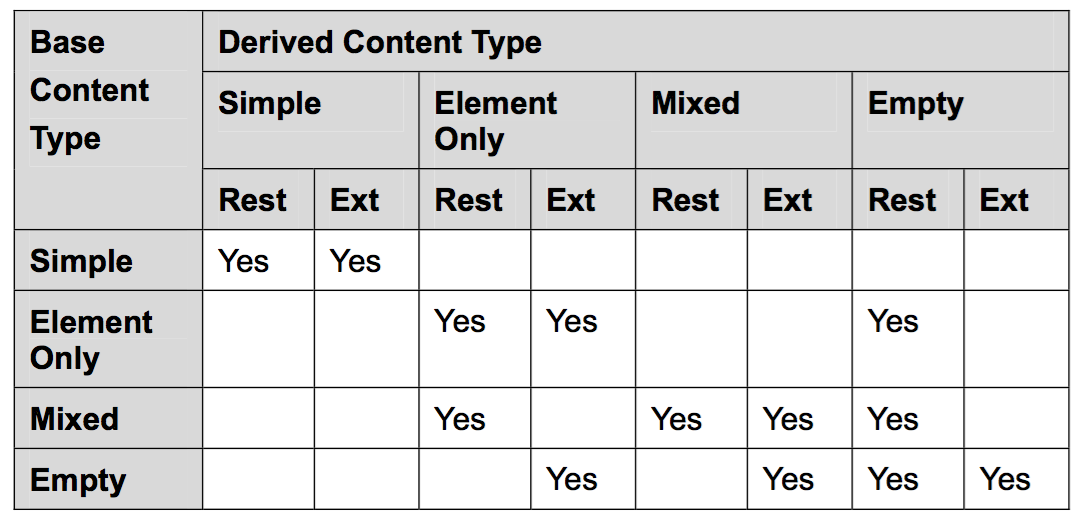
\includegraphics[width=.95\textwidth]{imgs/TabellaContentTypeDerivation.png}

	\end{block}

	\begin{tiny}
		\textit{Nuovi complex types possono essere creati a partire da altri complex types by extension and restriction.}
	\end{tiny}
\end{frame}



\begin{frame}
	\frametitle{Elementi per la definizione degli schemi xml}
	\framesubtitle{principi XSD}
	\addtocounter{nframe}{1}

	\begin{block}{Complex Type derivation: final attribute}
		\textbf{La derivazione di un tipo complesso può essere controllata impiegando l'attributo final nella dichiarazione del tipo}
	\end{block}

\end{frame}

\begin{frame}
	\frametitle{Elementi per la definizione degli schemi xml}
	\framesubtitle{principi XSD}
	\addtocounter{nframe}{1}

	\begin{block}{Complex Type derivation: final attribute}
		\textit{L'attributo final può assumere i seguenti valori:}
		\begin{itemize}
			\item \textbf{restriction}: limita la derivazione by restriction
			\item \textbf{extension}: limita la derivazione by extension
			\item \textbf{\#all}: limita la derivazione by restriction e by extension
		\end{itemize}

	\end{block}

\end{frame}

% esempio: how to control the derivation of a given complex type: 
\begin{frame}
	\frametitle{Elementi per la definizione degli schemi xml}
	\framesubtitle{principi XSD}
	\addtocounter{nframe}{1}

	\begin{block}{Complex Type derivation: esempio}

		\texttt{
			\emph{<xsd:complexType name=``ContactType'' final=``extension restriction''>}
			<xsd:sequence>
			<xsd:element name="Phone" minOccurs="0"/>
			</xsd:sequence>
			<xsd:attribute name="Name" />
			</xsd:complexType>
		}
	\end{block}
\end{frame}

\begin{frame}
	\frametitle{Elementi per la definizione degli schemi xml}
	\framesubtitle{principi XSD}
	\addtocounter{nframe}{1}

	\begin{block}{Complex Type derivation: esempio - derivazione non consentita}

		\texttt{
			<xsd:complexType name=``ExtendedContactType''>
			\emph{<xsd:complexContent>}
			\emph{<xsd:extension base="ContactType"/>}
			</xsd:complexContent>
			</xsd:complexType>
		}
	\end{block}
\end{frame}



\section{Introduzione Text Encoding Initiative}
%%Codifica di testi

% Le norme TEI
% Roberto Rosselli Del Turco
% Dipartimento di Studi Umanistici
% Università di Torino
% roberto.rossellidelturco@fileli.unipi.it
% roberto.rossellidelturco@unito.itLa codifica di testi – Le norme TEI
% La Text Encoding Initiative
% Sito WWW: http://www.tei-c.org/

\begin{frame}
	\frametitle{Intro Text Encoding Initiative}
	\framesubtitle{TEI}
	\addtocounter{nframe}{1}

	\begin{block}{Motto}
		TEI: Yesterday's information tomorrow
	\end{block}

	\begin{block}{Dal sito TEI}
		“an international and interdisciplinary standard that
		enables libraries, museums, publishers, and individual
		scholars to represent a variety of literary and linguistic
		texts for online research, teaching, and preservation”
	\end{block}
\end{frame}


\begin{frame}
	\frametitle{Intro Text Encoding Initiative}
	\framesubtitle{TEI}
	\addtocounter{nframe}{1}

	\begin{block}{testo di riferimento}
		Guidelines for Electronic Text Encoding and Interchange ( http://www.tei-c.org/Guidelines/ )
	\end{block}

	\begin{block}{testo di ausilio}
		BURNARD, Lou. What is the Text Encoding Initiative? How to add intelligent markup to digital resources. Nouva edizione [online]. Marseille: OpenEdition Press, 2014 (creato il 13 octobre 2018). Disponibile su Internet: <http://books.openedition.org/oep/426>. ISBN: 9782821834606. DOI: 10.4000/books.oep.426.

	\end{block}
\end{frame}


\begin{frame}
	\frametitle{Intro Text Encoding Initiative}
	\framesubtitle{TEI}
	\addtocounter{nframe}{1}

	\begin{block}{un po' di storia}
		\begin{itemize}
			\item 1987: necessità di standard che permetta la creazione e l’interscambio di documenti per mezzo di archivi informatici(convegno NY)
			\item 1990: prima versione delle Guidelines (TEI P1)
			\item 1990-94: fondi garantiti da enti quali NEH, Mellon Foundation, la Comunità Europea; supporto di ACH, ACL, ALLC
		\end{itemize}
	\end{block}

\end{frame}

\begin{frame}
	\frametitle{Intro Text Encoding Initiative}
	\framesubtitle{TEI}
	\addtocounter{nframe}{1}

	\begin{block}{un po' di storia}
		\begin{itemize}
			\item 2000: nascita del TEI Consortium, associazione non profit per lo sviluppo dello standard TEI
			\item 2002: passaggio da SGML a XML con la v. P4
			\item 2007: nuova versione TEI P5, continuamente aggiornata
		\end{itemize}
	\end{block}

\end{frame}


\begin{frame}
	\frametitle{Intro Text Encoding Initiative}
	\framesubtitle{TEI}
	\addtocounter{nframe}{1}

	\begin{block}{TEI Guidelines}
		\textit{versioni P1 – P3 basate su SGML}
		\\\textbf{versione P4}
		\begin{itemize}
			\item standard precedente, ancora impiegata
			\item basata su XML, DTD tradizionale
			\item pubblicata in forma definitiva nel 2002
			\item http://www.tei-c.org/Guidelines/P4/
		\end{itemize}
	\end{block}

\end{frame}

\begin{frame}
	\frametitle{Intro Text Encoding Initiative}
	\framesubtitle{TEI}
	\addtocounter{nframe}{1}

	\begin{block}{TEI Guidelines: versione P5}
		\begin{itemize}
			\item basata su XML, schema RelaxNG (e DTD tradizionale)
			\item pubblicata alla fine del 2007, aggiornata due volte l’anno
			\item molte novità interessanti (in particolare: maggior modularità)
			\item  http://www.tei-c.org/Guidelines/P5/
		\end{itemize}
	\end{block}

\end{frame}

\begin{frame}
	\frametitle{Intro Text Encoding Initiative}
	\framesubtitle{TEI}
	\addtocounter{nframe}{1}

	\begin{block}{TEI Guidelines: Obiettivi}
		\begin{itemize}
			\item better interchange and integration of scholarly data
			\item support for all texts, in all languages, from all periods
			\item guidance for the perplexed: what to encode - hence, a user-driven codification of existing best practice
			\item assistance for the specialist: how to encode --- hence, a loose framework into which unpredictable extensions can be fitted
		\end{itemize}
	\end{block}

\end{frame}



\begin{frame}
	\frametitle{Intro Text Encoding Initiative}
	\framesubtitle{TEI}
	\addtocounter{nframe}{1}

	\begin{block}{TEI Guidelines: Obiettivi}
		These apparently incompatible goals result in a highly flexible,
		modular, environment for DTD customization.
		Lou Burnard, TEI and XML: a marriage made in heaven?
		(http://www.tei-c.org/Talks/marriage.xml?style=printable)
	\end{block}

\end{frame}


\begin{frame}
	\frametitle{Intro Text Encoding Initiative}
	\framesubtitle{TEI}
	\addtocounter{nframe}{1}

	\begin{block}{Che cosa offre la TEI}
		% un ricco (e complesso) manuale di codifica, le Guidelines
		% for Electronic Text Encoding and Interchange, che
		% comprende un numero elevato di elementi, sia di tipo
		% strutturale sia semantico, definiti per mezzo di
		% un certo numero di schemi di codifica (DTD o schema
		% language) che sono
		% organizzati in una struttura altamente modulare e
		% personalizzabile.

	\end{block}

\end{frame}

\begin{frame}
	\frametitle{Intro Text Encoding Initiative}
	\framesubtitle{TEI}
	\addtocounter{nframe}{1}

	\begin{block}{Che cosa offre la TEI}
		\begin{itemize}
			\item \textbf{è possibile scegliere soltanto i moduli necessari}
			\item \textbf{è possibile modificare le definizioni degli elementi}
		\end{itemize}

	\end{block}

\end{frame}



\begin{frame}
	\frametitle{Intro Text Encoding Initiative}
	\framesubtitle{TEI}
	\addtocounter{nframe}{1}

	\begin{block}{Supporto per gli utenti}
		\begin{itemize}
			\item il sito del consorzio (http://www.tei-c.org/)
			\item pagine relative alle varie versioni delle Guidelines
			\item software, tutorial, etc.
			\item il wiki: http://www.tei-c.org/wiki/index.php/Main_Page
			\item la mailing list TEI-L
			\item Github: https://github.com/TEIC
			\item TEI by example: http://teibyexample.org/
		\end{itemize}

	\end{block}

\end{frame}


\begin{frame}
	\frametitle{Intro Text Encoding Initiative}
	\framesubtitle{TEI}
	\addtocounter{nframe}{1}

	\begin{block}{Novità della versione P5}
		\begin{itemize}
			\item modulo di descrizione dei manoscritti
			\item grafica e multimedia
			\item standoff markup
			\item supporto per i namespace XML
			\item miglioramenti nel modulo feature structure
			\item miglioramenti (limitati ...) nella gestione di varianti testuali
			\item nuovi meccanismi di linking
			\item personalizzazione semplificata
			\item varie migliorie tecniche
		\end{itemize}

	\end{block}

\end{frame}


\begin{frame}
	\frametitle{Intro Text Encoding Initiative}
	\framesubtitle{TEI}
	\addtocounter{nframe}{1}

	\begin{block}{TEI: Struttura modulare}
		\begin{itemize}
			\item si scelgono soltanto i moduli che corrispondono alle proprie esigenze, in modo da realizzare rapidamente uno schema di codifica appropriato
			\item ogni modulo contiene un certo numero di elementi (tagset)
			\item gli elementi sono organizzati in classi (strutturali,semantiche)
			\item gli attributi sono organizzati in classi (globali e specifici)
		\end{itemize}

	\end{block}

\end{frame}


% classi strutturali: elementi che hanno un ruolo a livello strutturale
% (paragrafi, strofe, etc.)
% classi semantiche: elementi descrittivi del testo (aggiunte,
% correzioni, nomi di persona, etc.)
% anche gli attributi sono organizzati in classi
% attributi globali: disponibili per tutti gli elementi
% attributi specifici: solo per alcuni elementi


\begin{frame}
	\frametitle{Intro Text Encoding Initiative}
	\framesubtitle{TEI}
	\addtocounter{nframe}{1}

	\begin{block}{TEI: Struttura modulare - Moduli essenziali}
		\begin{itemize}
			\item \textbf{tei}: definisce le classi di elementi, le macro e i datatype che verranno usati per tutti i moduli
			\item \textbf{header}: l’intestazione contenente i metadati relativi al documento TEI XML
			\item \textbf{textstructure}: elementi strutturali per qualsiasi tipo di testo
			\item \textbf{core}: elementi utili in qualsiasi tipo di documento
		\end{itemize}

	\end{block}

\end{frame}

\begin{frame}
	\frametitle{Intro Text Encoding Initiative}
	\framesubtitle{TEI}
	\addtocounter{nframe}{1}

	\begin{block}{TEI: Struttura modulare - Moduli facoltativi}
		\begin{itemize}
			\item \textbf{analysis}: strumenti per analisi (linguistica etc.) del testo
			\item \textbf{corpus}: gestione di corpora linguistici
			\item \textbf{drama}: elementi per testi teatrali e drammatici
			\item \textbf{gaiji}: rappresentazione di caratteri e glifi non standard
			\item \textbf{msdescription}: metadati relativi a manoscritti
			\item \textbf{spoken}: trascrizione del parlato
			\item \textbf{textcrit}: apparato critico
			\item \textbf{transcr}:  trascrizione di fonti primarie (manoscritti)
			\item \textbf{verse}: elementi supplementari per testi poetici
		\end{itemize}

	\end{block}

\end{frame}

\begin{frame}
	\frametitle{Intro Text Encoding Initiative}
	\framesubtitle{TEI}
	\addtocounter{nframe}{1}

	\begin{block}{TEI: Struttura modulare - Moduli}

		\textbf{SITO TEI PER ELENCP MODULI}

	\end{block}

\end{frame}


\begin{frame}
	\frametitle{Intro Text Encoding Initiative}
	\framesubtitle{TEI}
	\addtocounter{nframe}{1}

	\begin{block}{TEI Lite}

		una specifica \textbf{personalizzazione} della TEI versione P4/5

	\end{block}

	\textit{a simple demonstration of how the TEI encoding scheme
		might be adopted to meet 90\% of the needs of 90\% of the
		TEI user community (dalla Prefatory Note: http://www.tei-
		c.org/Lite/)}

\end{frame}


\begin{frame}
	\frametitle{Intro Text Encoding Initiative}
	\framesubtitle{TEI}
	\addtocounter{nframe}{1}

	\begin{block}{TEI Lite}

		la versione P4 è stata tradotta anche in italiano: TEI Lite:
		introduzione alla codifica dei testi, a cura di F. Ciotti (
		http://www.tei-c.org/Lite/teiu5_it.html)
		molto usata, ma presenta varie limitazioni
		con la versione P5 è più semplice produrre una versione
		semplificata o personalizzata

	\end{block}


\end{frame}

\begin{frame}
	\frametitle{Intro Text Encoding Initiative}
	\framesubtitle{TEI}
	\addtocounter{nframe}{1}

	\begin{block}{TEI Pizza chef}

		la TEI P4 poteva essere modificata usando un programma su
		web chiamato Pizza chef
		http://www.tei-c.org.uk/pizza.html
		metafora della base e dei condimenti (toppings),
		corrispondenti ai moduli indispensabili e a quelli facoltativi
		meccanismo efficace, soprattutto considerando l’alternativa
		(modifica manuale delle DTD TEI), ma obsoleto
		necessaria comunque modifica manuale per nuovi elementi

	\end{block}


\end{frame}

\begin{frame}
	\frametitle{Intro Text Encoding Initiative}
	\framesubtitle{TEI}
	\addtocounter{nframe}{1}

	\begin{block}{TEI Roma}

		per la P5 si è deciso di proporre una modularizzazione più
		efficace, e uno strumento di personalizzazione più potente.
		Strumento basato sul nuovo formato ODD.


	\end{block}

	\begin{block}{TEI Roma}
		il metodo da seguire per la versione P5 (quella che
		useremo) fino all’arrivo del successore (Byzantium)

	\end{block}

\end{frame}

\begin{frame}
	\frametitle{Intro Text Encoding Initiative}
	\framesubtitle{TEI}
	\addtocounter{nframe}{1}

	\begin{block}{TEI Roma}

		\begin{itemize}
			\item  possibilità di scegliere, escludere, modificare sia gli elementi (e le classi di elementi), sia gli attributi (e le classi di attributi)
			\item possibilità di aggiungere elementi (eventualmente inserendoli nelle classi preesistenti)
			\item possibilità di salvare lo schema in tre formati diversi: DTD  tradizionale, W3C e RelaxNG (anche in forma compatta)
		\end{itemize}

	\end{block}


\end{frame}


\begin{frame}
	\frametitle{Intro Text Encoding Initiative}
	\framesubtitle{TEI}
	\addtocounter{nframe}{1}

	\begin{block}{TEI Roma: Il formato ODD}
		le versioni P1 – P4 delle DTD TEI erano nel formato DTD language e dipendevano dalla sintassi SGML per molti aspetti
	\end{block}

	\begin{block}{TEI Roma: Il formato ODD}
		One Document Does it all (ODD): set di specifiche in base alle quali un semplice documento TEI XML “defines a schema in terms of the modules it requires, together with any possible modifications, such as the desired
		root element” risultato finale: lo schema nel linguaggio desiderato e la relativa documentazione
	\end{block}

\end{frame}


\begin{frame}
	\frametitle{Intro Text Encoding Initiative}
	\framesubtitle{TEI}
	\addtocounter{nframe}{1}

	\begin{block}{TEI Roma: Il formato ODD}

		tutorial: Getting Started with P5 ODDs\\
		http://www.tei-c.org/Guidelines/Customization/odds.xml

	\end{block}


\end{frame}


% 15La codifica di testi – Le norme TEI
% TEI Roma 2
% per motivi vari, la manutenzione di TEI Roma lascia a
% desiderare (per non parlare dello sviluppo di un successore)
% nel passato recente la componente di “controllo” dello
% schema (Sanity checker) non funzionava
% in tal caso è possibile andare sul sito TEI di Oxford dove è in
% esecuzione una versione più vecchia:
% http://tei.it.ox.ac.uk/Roma/
% Roma, in ogni caso, è solo un front-end per il linguaggio ODD
% (cfr. infra)




\begin{frame}
	\frametitle{Intro Text Encoding Initiative}
	\framesubtitle{TEI}
	\addtocounter{nframe}{1}

	\begin{block}{Il futuro della TEI}
		\textbf{negli ultimi anni gli schemi TEI sono stati oggetto di alcune critiche}
	\end{block}

	\begin{block}{Il futuro della TEI}
		\begin{itemize}
			\item la TEI è troppo grande / complicata / piccola
			\item la TEI è basata su XML e questo formato è in declino
			\item la TEI/XML non supporta le gerarchie multiple
			\item la TEI non supporta il markup di tipo stand-off
		\end{itemize}
	\end{block}

\end{frame}


\begin{frame}
	\frametitle{Intro Text Encoding Initiative}
	\framesubtitle{TEI}
	\addtocounter{nframe}{1}

	\begin{block}{Il futuro della TEI}
		\textbf{negli ultimi anni gli schemi TEI sono stati oggetto di alcune critiche}
	\end{block}

	\begin{block}{Il futuro della TEI}
		la cosa importante da ricordare è che il formato XML non è
		la TEI (in passato SGML, in futuro chissà → abstraction level)
		al contrario, se c’è una discrepanza fra Guidelines e schemi,
		la precedenza va alle Guidelines
	\end{block}

\end{frame}


\begin{frame}
	\frametitle{Intro Text Encoding Initiative}
	\framesubtitle{TEI}
	\addtocounter{nframe}{1}

	\begin{block}{text encoding con la TEI}
		è caldamente raccomandato usare direttamente la
		versione più recente della P5.\\
		La flessibilità della P5 permette di definire uno schema di
		codifica che corrisponda precisamente al modello
    \end{block}
    
    \textit{La comunità di utenti e sviluppatori TEI offre un buon supporto.}

\end{frame}




%%%%%%%%%%%%%%%%%%%%%%
% Codifica di testi
% I moduli base della TEI
% Roberto Rosselli Del Turco
% Dipartimento di Studi Umanistici
% Università di Torino
% roberto.rossellidelturco@fileli.unipi.it
% roberto.rossellidelturco@unito.itSchemi di codifica TEI – Moduli base
% Elementi disponibili per tutti i documenti TEI

\begin{frame}
	\frametitle{Intro Text Encoding Initiative}
	\framesubtitle{TEI}
	\addtocounter{nframe}{1}

	\begin{block}{TEI}
        un documento TEI P5 ‘minimo’ è composto da :
        intestazione XML
        intestazione TEI
        elementi strutturali
        elementi semantici dei moduli base (non indispensabili)
        anche usando soltanto i moduli essenziali si ha a disposizione
        uno schema adatto alla marcatura di numerosi tipi di testi
        moduli di base: tei, header, textstructure, core
        schemi ‘leggeri’ consigliati: la TEI Lite, o se necessario una
        versione personalizzata e ancora più ridotta della P5 (TEI
        Absolutely Bare)
    \end{block}
    
   

\end{frame}




begin{frame}
	\frametitle{Intro Text Encoding Initiative}
	\framesubtitle{TEI}
	\addtocounter{nframe}{1}

	\begin{block}{TEI}
        2Schemi di codifica TEI – Moduli base
        Nota sugli elementi spiegati
        punto di riferimento per il corso: la TEI P5 “completa”
        iniziamo con la TEI Lite (= versione “leggera”)
        proposti elementi di uso generale e di uso specifico
        per cominciare, la TEI Lite è più semplice da gestire
        elementi non presenti di default evidenziati in rosso scuro
        in caso di dubbio consultare le liste degli elementi:
        TEI Lite: http://www.tei-c.org/release/doc/tei-p5-exemplars/html/teilite.doc.html
        TEI P5: http://www.tei-c.org/release/doc/tei-p5-doc/en/html/REF-ELEMENTS.html
        NB: quando si crea lo schema controllare che gli elementi
        siano effettivamente inclusi nei moduli prescelti
    \end{block}
    
   

\end{frame}



begin{frame}
	\frametitle{Intro Text Encoding Initiative}
	\framesubtitle{TEI}
	\addtocounter{nframe}{1}

	\begin{block}{TEI}
        3Schemi di codifica TEI – Moduli base
        Caratteristiche degli elementi spiegati
        gli elementi TEI rientrano nelle categorie generali di
        elementi XML che abbiamo visto in precedenza:
        elementi che possono contenere solo altri elementi (=
        elementi strutturali)
        elementi che possono contenere altri elementi e testo
        elementi che possono contenere solo testo
        elementi vuoti (es. <pb/>)
        gli elementi vuoti marcano una gerarchia differente
        NB: inserire il contenuto sbagliato (ad es. testo in un
        elemento strutturale) significa rendere non valido il
        documento TEI
    \end{block}
    
   

\end{frame}






begin{frame}
	\frametitle{Intro Text Encoding Initiative}
	\framesubtitle{TEI}
	\addtocounter{nframe}{1}

	\begin{block}{TEI}
        4Schemi di codifica TEI – Moduli base
        Gerarchie multiple 1
        <?xml version="1.0" encoding="utf-8"?>
        <text>
        <titolo>Gli assassinii della Rue Morgue</titolo>
        <intestazione> I </intestazione>
        <pagina n="5">
        <p>Le facoltà mentali che si sogliono chiamare analitiche sono, di
        per se stesse, poco suscettibili di analisi. Le conosciamo soltanto negli
        effetti. [...]</p>
        <p>La facoltà di risolvere è probabilmente molto rinfor-
        </pagina>
        <pagina n="6">
        zata dallo studio delle matematiche e in modo particolare
        dell’altissimo ramo di questa scienza che – impropriamente e solo in
        ragione delle sue operazioni in senso retrogrado – è stata chiamata
        analisi [...] </p>
        </pagina>
        </text>
    \end{block}
    
   

\end{frame}






begin{frame}
	\frametitle{Intro Text Encoding Initiative}
	\framesubtitle{TEI}
	\addtocounter{nframe}{1}

	\begin{block}{TEI}
        5Schemi di codifica TEI – Moduli base
        Gerarchie multiple 2: elementi vuoti
        <?xml version="1.0" encoding="utf-8"?>
        <text>
        <titolo>Gli assassinii della Rue Morgue</titolo>
        <intestazione> I </intestazione>
        <pagina n="5"/>
        <p>Le facoltà mentali che si sogliono chiamare analitiche sono, di
        per se stesse, poco suscettibili di analisi. Le conosciamo soltanto negli
        effetti. [...]</p>
        <p>La facoltà di risolvere è probabilmente molto rinfor-
        <pagina n="6"/>
        zata dallo studio delle matematiche e in modo particolare
        dell’altissimo ramo di questa scienza che – impropriamente e solo in
        ragione delle sue operazioni in senso retrogrado – è stata chiamata
        analisi [...] </p>
        </text>
    \end{block}
    
   

\end{frame}






begin{frame}
	\frametitle{Intro Text Encoding Initiative}
	\framesubtitle{TEI}
	\addtocounter{nframe}{1}

	\begin{block}{TEI}
        6Schemi di codifica TEI – Moduli base
        Struttura di un documento TEI
        struttura fondamentale all’interno della radice (<TEI>):
        una intestazione TEI (<teiHeader>)
        un testo: <text> (o più testi, cfr. infra)
        contenuto del TEI header:
        metadati relativi al documento (utili per collezioni di testi
        codificati)
        descrizione del file usando <fileDesc> (obbligatoria)
        descrizioni relative al tipo di codifica, al contenuto del
        documento, alle sue revisioni (facoltative)
        è possibile includere testi introduttivi e spiegazioni relative alla
        codifica effettuata (preziosi per l’interscambio!)
    \end{block}
    
   

\end{frame}






begin{frame}
	\frametitle{Intro Text Encoding Initiative}
	\framesubtitle{TEI}
	\addtocounter{nframe}{1}

	\begin{block}{TEI}
        7Schemi di codifica TEI – Moduli base
        Esempio 1
        <?xml version="1.0" encoding="utf-8"?>
        <!DOCTYPE TEI SYSTEM "tei_lite.dtd">
        <TEI xmlns="http://www.tei-c.org/ns/1.0">
        <teiHeader>...</teiHeader>
        <text>
        <div>
        <p></p>
        </div>
        </text>
        </TEI>
    \end{block}
    
   

\end{frame}






begin{frame}
	\frametitle{Intro Text Encoding Initiative}
	\framesubtitle{TEI}
	\addtocounter{nframe}{1}

	\begin{block}{TEI}
        8Schemi di codifica TEI – Moduli base
        Esempio 2
        <?xml version="1.0" encoding="utf-8"?>
        <?xml-model href="tei-lite.rng"?>
        <TEI xmlns="http://www.tei-c.org/ns/1.0">
        <teiHeader>...</teiHeader>
        <text>
        <div>
        <p></p>
        </div>
        </text>
        </TEI>
    \end{block}
    
   

\end{frame}






begin{frame}
	\frametitle{Intro Text Encoding Initiative}
	\framesubtitle{TEI}
	\addtocounter{nframe}{1}

	\begin{block}{TEI}
        9Schemi di codifica TEI – Moduli base
        Struttura di un documento TEI
        schema di intestazione TEI minima:
        <teiHeader>
        <fileDesc>
        <titleStmt>...</titleStmt>
        <publicationStmt>...</publicationStmt>
        <sourceDesc>...</sourceDesc>
        </fileDesc>
        </teiHeader>
        metadati essenziali riguardo il titolo, la modalità di diffusione e
        la fonte originaria di un testo codificato
        permettono classificazione, archiviazione ed elaborazione
        bibliografica
    \end{block}
    
   

\end{frame}





begin{frame}
	\frametitle{Intro Text Encoding Initiative}
	\framesubtitle{TEI}
	\addtocounter{nframe}{1}

	\begin{block}{TEI}
        10Schemi di codifica TEI – Moduli base
        Esempio di intestazione TEI
        <teiHeader>
        <fileDesc>
        <titleStmt>
        <title>La Divina Commedia: versione elettronica</title>
        <respStmt>
        <resp>Conversione TEI P5 a cura di</resp><name>M. Rossi</name>
        </respStmt>
        </titleStmt>
        <publicationStmt>
        <publisher>Università di Pisa</publisher>
        <date>2002-11-07</date>
        <availability status="restricted"><p>Contattare il responsabile del
        progetto, vietata la riproduzione.</p></availability>
        </publicationStmt>
        <sourceDesc>
        <bibl><title>La Divina Commedia</title><author>Dante Alighieri
        </author><publisher>Mondadori</publisher><date>1988</date></bibl>
        </sourceDesc>
        </fileDesc>
        </teiHeader>
    \end{block}
    
   

\end{frame}






begin{frame}
	\frametitle{Intro Text Encoding Initiative}
	\framesubtitle{TEI}
	\addtocounter{nframe}{1}

	\begin{block}{TEI}
        11Schemi di codifica TEI – Moduli base
        Struttura di un documento TEI
        le altre componenti dell’intestazione TEI:
        <encodingDesc> informazioni riguardo lo schema (e il
        modello di codifica) utilizzato
        <profileDesc>
        descrizione del testo: quando è stato
        creato, da chi, usando quali lingue etc.
        <revisionDesc> informazioni sulle versioni del file
        stesso livello di <fileDesc>, vedremo con più dettagli
        i metadati sono una componente essenziale di qualsiasi
        progetto di digitalizzazione
    \end{block}
    
   

\end{frame}






begin{frame}
	\frametitle{Intro Text Encoding Initiative}
	\framesubtitle{TEI}
	\addtocounter{nframe}{1}

	\begin{block}{TEI}
        12Schemi di codifica TEI – Moduli base
        Elementi strutturali
        <text>
        un singolo testo di qualsiasi tipo
        punto di partenza della gerarchia riguardo il contenuto
        può essere affiancato o sostituito da <facsimile>
        all’interno di <text> possiamo trovare quattro elementi:
        <front> materiale che precede il testo (se presente)
        <body> il testo stesso
        <back> materiale che segue il testo (se presente)
        <group> alternativo a <body>, raggruppa testi diversi
    \end{block}
    
   

\end{frame}







begin{frame}
	\frametitle{Intro Text Encoding Initiative}
	\framesubtitle{TEI}
	\addtocounter{nframe}{1}

	\begin{block}{TEI}
        13Schemi di codifica TEI – Moduli base
        Struttura di un documento TEI
        esempio schematico di documento TEI unitario:
        <TEI>
        <teiHeader> [informazioni del TEI Header]
        </teiHeader>
        <text>
        <front> [premessa, dedica ...] </front>
        <body> [corpo del testo ...] </body>
        <back> [postfazione, appendice ...]</back>
        </text>
        </TEI>
    \end{block}
    
   

\end{frame}






begin{frame}
	\frametitle{Intro Text Encoding Initiative}
	\framesubtitle{TEI}
	\addtocounter{nframe}{1}

	\begin{block}{TEI}
        14Schemi di codifica TEI – Moduli base
        Struttura di un documento TEI
        è possibile costruire documenti compositi:
        rimpiazzando il <body> con un gruppo (<group>) di testi si
        ottiene un documento composito
        ciascuno di questi testi è rappresentato secondo la struttura
        vista prima
        un’altra possibilità è creare un corpus con <teiCorpus>:
        intestazioni (<teiHeader>) separate per il corpus e per
        ciascun gruppo di testi
        struttura più complessa, su più livelli
    \end{block}
    
   

\end{frame}







begin{frame}
	\frametitle{Intro Text Encoding Initiative}
	\framesubtitle{TEI}
	\addtocounter{nframe}{1}

	\begin{block}{TEI}
        15Schemi di codifica TEI – Moduli base
        Schema di testo composito
        <TEI>
        <teiHeader> [ intestazione del testo composito ] </teiHeader>
        <text>
        <front> [ front matter del composito ] </front>
        <group>
        <text>
        <front> [ front matter del primo testo ] </front>
        <body> [ body del primo testo ]
        </body>
        <back> [ back matter del primo testo ] </back>
        </text>
        <text>
        <front> [ front matter del secondo testo] </front>
        <body> [ body del secondo testo ]
        </body>
        <back> [ back matter del secondo testo ] </back>
        </text>
        ...
        [ altri testi o gruppi di testi ]
        ...
        </group>
        <back>
        [ back matter del composito ]
        </back>
        </text>
        </TEI>
    \end{block}
    
   

\end{frame}







begin{frame}
	\frametitle{Intro Text Encoding Initiative}
	\framesubtitle{TEI}
	\addtocounter{nframe}{1}

	\begin{block}{TEI}
	% 16Schemi di codifica TEI – Moduli base
% Costruzione di corpora TEI
% esempio schematico di TEI Corpus:
% <teiCorpus>
% <teiHeader> [metadati per il corpus] </teiHeader>
% <TEI>
% <teiHeader> [metadati relativi al I testo]</teiHeader>
% <text> [primo testo del corpus] </text>
% </TEI>
% <TEI>
% <teiHeader>[metadati relativi al II testo]</teiHeader>
% <text> [secondo testo del corpus] </text>
% </TEI>
% </teiCorpus>
    \end{block}
    
   

\end{frame}





begin{frame}
	\frametitle{Intro Text Encoding Initiative}
	\framesubtitle{TEI}
	\addtocounter{nframe}{1}

	\begin{block}{TEI}
	 17Schemi di codifica TEI – Moduli base
 CONTROLLARE IMMAGINE
    \end{block}
    
   

\end{frame}





begin{frame}
	\frametitle{Intro Text Encoding Initiative}
	\framesubtitle{TEI}
	\addtocounter{nframe}{1}

	\begin{block}{TEI}
        18Schemi di codifica TEI – Moduli base
        Altri elementi strutturali fondamentali
        suddivisioni del testo:
        non numerati: <div> (nessun limite di nidificazione)
        numerati: <div1> ... <div7> (massimo 7 livelli)
        paragrafi: <p>
        testo riferito: <q> (discorso diretto, citazioni, etc.)
        versi: strofe <lg> e singoli versi <l>
        testi teatrali: discorsi <sp> che possono contenere paragrafi
        <p> o versi <l>, oltre a direzioni di scena <stage>
        milestone tags: <pb/>, <lb/>, <cb/>, <milestone/>
        notare che un <div> può contenere un <floatingText>:
        possibilità di introdurre gerarchie complesse
    \end{block}
    
   

\end{frame}



begin{frame}
	\frametitle{Intro Text Encoding Initiative}
	\framesubtitle{TEI}
	\addtocounter{nframe}{1}

	\begin{block}{TEI}
        19Schemi di codifica TEI – Moduli base
        Apertura e chiusura di un <div>
        <head>
        qualunque tipo di intestazione: il titolo di un opera,
        l’intestazione di un paragrafo, di una sezione, etc.
        type
        permette di classificare in base a una tipologia
        <epigraph> citazione all’inizio del testo, o nella pagina del titolo,
        eventualmente con riferimento bibliografico
        <opener> raggruppa un serie di elementi (data, luogo, saluti,
        etc.) all’inizio del <div>, specie di una lettera
        <argument> lista degli argomenti trattati nel <div>
        <trailer>
        frase che compare alla fine del <div> (ad esempio
        “Fine del capitolo 1”)
        <closer>
        raggruppa un serie di elementi (data, luogo, saluti,
        etc.) alla fine del <div>, specie di una lettera
    \end{block}
    
   

\end{frame}




begin{frame}
	\frametitle{Intro Text Encoding Initiative}
	\framesubtitle{TEI}
	\addtocounter{nframe}{1}

	\begin{block}{TEI}
        20Schemi di codifica TEI – Moduli base
        Esempio di <div> con apertura/chiusura
        <div type="lettera”>
        <opener>
        <dateline>
        <name type="place">Pisa</name>
        <date>20 marzo 2015</date>
        </dateline>
        <salute>Gentilissima Prof.ssa Scannagatti,</salute>
        </opener>
        <p>sono spiacente di doverle comunicare che un’invasione di cavallette si
        è abbattuta sui miei quaderni incautamente lasciati in giardino, e li ha
        divorati interamente.</p>
        <p>Questo purtroppo significa che non posso mostrare i compiti svolti,
        come sempre, con solerzia e assiduo impegno.</p>
        <closer>
        <salute>Certo di poter contare sulla sua comprensione le porgo i miei
        migliori saluti,</salute>
        <signed>Pierino Rossi</signed>
        </closer>
        </div>
    \end{block}
    
   

\end{frame}





begin{frame}
	\frametitle{Intro Text Encoding Initiative}
	\framesubtitle{TEI}
	\addtocounter{nframe}{1}

	\begin{block}{TEI}
        21Schemi di codifica TEI – Moduli base
        Errori frequenti 1
        molto spesso nell’intestazione si fraintende il significato
        dell’elemento <fileDesc>
        questo elemento serve in primo luogo a dare informazioni
        sul file stesso, non sul testo originale
        il riferimento alla fonte dalla quale è tratto il testo codificato
        deve essere inserito nel <sourceDesc>
        i titoli sono codificati con <title> soltanto nel caso di
        riferimenti bibliografici
        i titoli del testo, dei capitoli etc. si marcano con <head>
    \end{block}
    
   

\end{frame}





begin{frame}
	\frametitle{Intro Text Encoding Initiative}
	\framesubtitle{TEI}
	\addtocounter{nframe}{1}

	\begin{block}{TEI}
        22Schemi di codifica TEI – Moduli base
        Nota sugli errori possibili
        gli errori che si possono commettere durante la codifica
        di un testo ricadono più o meno in tre categorie:
        errori sintattici: un elemento inserito in un punto sbagliato
        della gerarchia, o che non può contenere testo etc.
        errori di marcatura semantica: usare un elemento inadatto
        allo scopo, ad esempio marcare un titolo con <emph>
        errori di interpretazione del testo (che portano al II tipo o
        all’assenza del markup che andrebbe inserito)
        gli errori del primo tipo sono i più facili da individuare e
        correggere, quelli del terzo i più difficili
    \end{block}
    
   

\end{frame}





begin{frame}
	\frametitle{Intro Text Encoding Initiative}
	\framesubtitle{TEI}
	\addtocounter{nframe}{1}

	\begin{block}{TEI}
        23Schemi di codifica TEI – Moduli base
        A proposito di <div>
        domanda che ricorre periodicamente: perché non usare nomi
        più significativi invece di un contenitore generico come <div>
        (= ‘suddivisione, parte di un testo’)?
        perché non usare <book>, <chapter>, <section>, etc. come
        fa, ad esempio, lo schema DOCBOOK?
        troppa variabilità nell’uso comune, meglio usare un termine
        generico che possa poi essere specificato usando l’attributo
        type (es. <div type=”chapter”>)
        i <div>, numerati o meno, possono essere ‘nidificati’, nessun
        problema nel riproporre la struttura editoriale visibile
    \end{block}
    
   

\end{frame}





begin{frame}
	\frametitle{Intro Text Encoding Initiative}
	\framesubtitle{TEI}
	\addtocounter{nframe}{1}

	\begin{block}{TEI}
        24Schemi di codifica TEI – Moduli base
        Attributi globali
        alcuni attributi possono essere usati con qualsiasi
        elemento (v. la classe att.global), in particolare:
        n
        un numero o un nome non univoco, possibilmente breve,
        per identificare un elemento
        rend informazioni relative all’aspetto (originale!) del testo
        rendition simile a @rend, ma fa riferimento a elementi
        <rendition> inseriti nell’<encodingDesc> (dentro <tagsDecl>)
        xml:lang la lingua del testo contenuto da un elemento
        xml:id un identificatore univoco per l’elemento
        NB: in base ai moduli usati nello schema sono disponibili ulteriori attributi globali
    \end{block}
    
   

\end{frame}





begin{frame}
	\frametitle{Intro Text Encoding Initiative}
	\framesubtitle{TEI}
	\addtocounter{nframe}{1}

	\begin{block}{TEI}
        25Schemi di codifica TEI – Moduli base
        Esempio 1
        <text>
        <body>
        <div n="ch1" type="chapter">
        <pb n="1"/>[...]
        <p>[...] risulta chiaro se avete letto <title
        rend="underline" xml:lang="fra">Les fleurs du
        mal</title> [...]</p>
        <p>[...] un grande esempio di <foreign
        xml:lang="fra">savoir faire</foreign> [...]</p>
        [...]
        </div>
        [ altri div ... ]
        </body>
        </text>
    \end{block}
    
   

\end{frame}





begin{frame}
	\frametitle{Intro Text Encoding Initiative}
	\framesubtitle{TEI}
	\addtocounter{nframe}{1}

	\begin{block}{TEI}
        26Schemi di codifica TEI – Moduli base
        Esempio 2
        <text>
        <body>
        <div n="ch1" type="chapter"> <pb n="1"/> [...]
        <p n="1">[...] descritto altrove (si veda ad
        esempio <ref target="#Rossi94">Rossi 1994</ref>)
        [...] </p> [...]
        </div>
        [ altri div ... ]
        <div n="bib" type="bibliography">
        [...]
        <bibl xml:id="Rossi94">
        <author>Rossi, M.</author>[...]</bibl>
        [...]
        </div>
        </body>
        </text>
    \end{block}
    
   

\end{frame}





begin{frame}
	\frametitle{Intro Text Encoding Initiative}
	\framesubtitle{TEI}
	\addtocounter{nframe}{1}

	\begin{block}{TEI}
        27Schemi di codifica TEI – Moduli base
        Esercizio 1
        marcare il testo (file ese01.txt) come segue:
        editor da usare: XML Copy Editor
        inserire intestazione XML
        marcare la struttura usando gli elementi fin qui descritti
        in particolare marcare tutti i paragrafi usando <p>
        verificare che sia ben formato premendo F2
        salvare il file XML come ese01-Cognome.xml
        file nominati diversamente non saranno accettati
        testi tratti da http://www.liberliber.it/
    \end{block}
    
   

\end{frame}





begin{frame}
	\frametitle{Intro Text Encoding Initiative}
	\framesubtitle{TEI}
	\addtocounter{nframe}{1}

	\begin{block}{TEI}
        28Schemi di codifica TEI – Moduli base
        Suggerimenti riguardo gli esercizi
        non fate copia e incolla da Wordpad o Notepad, aprite
        direttamente i testi usando XML Copy editor
        i documenti XML hanno come estensione .xml, quindi
        salvate subito una copia con tale estensione
        aprite le Guidelines TEI nel navigatore
        per prima cosa marcare la struttura: cominciare la
        marcatura semantica come secondo passo
        ogni esercizio ha degli obiettivi da raggiungere:
        controllate prima di spedire
        non lasciate accumulare gli errori
    \end{block}
    
   

\end{frame}



begin{frame}
	\frametitle{Intro Text Encoding Initiative}
	\framesubtitle{TEI}
	\addtocounter{nframe}{1}

	\begin{block}{TEI}
        29Schemi di codifica TEI – Moduli base
        Errori frequenti 2
        <div> non può essere usato allo stesso livello gerarchico
        di <p>, in altre parole non si può alternare <div> con
        <p>:
        <div> [...] </div>
        <p> [...] </p>
        <div> [...] </div>
        ← INVALID!!!
        <div> e tutti gli altri elementi strutturali “puri” non
        possono contenere testo:
        <div>Pippo</div>
        ← INVALID!!!
        <person>Pippo</person> ← INVALID!!!
    \end{block}
    
   

\end{frame}






begin{frame}
	\frametitle{Intro Text Encoding Initiative}
	\framesubtitle{TEI}
	\addtocounter{nframe}{1}

	\begin{block}{TEI}
        30Schemi di codifica TEI – Moduli base
        Enfasi e termini particolari 1
        <emph>
        parole o frasi enfatizzate nel testo
        questo è il <emph>mio</emph> computer!
        <foreign>
        parola o frase in una lingua diversa
        In quel punto entrò il bidello a dare il <foreign
        xml:lang="lat">finis</foreign>.
        <distinct>
        “diverso” dal testo (arcaico, gergale, etc.)
        saltò in groppa al <distinct>fido destriero</distinct>
        <hi>
        elemento generico
        <hi rend="double">N</hi>el mezzo del cammin di nostra vita
        il suo nome è <hi rend="italic">Mario Rossi</hi>
    \end{block}
    
   

\end{frame}




begin{frame}
	\frametitle{Intro Text Encoding Initiative}
	\framesubtitle{TEI}
	\addtocounter{nframe}{1}

	\begin{block}{TEI}
        31Schemi di codifica TEI – Moduli base
        Enfasi e termini particolari 2
        <mentioned> parola o frase menzionata ma non usata
        il termine corretto è <mentioned>epigrafe</mentioned>
        <soCalled>
        parola o espressione da cui ci si distanzia
        il cosiddetto <soCalled>darwinismo sociale</soCalled>
        <term>
        una o più parole considerate termine tecnico
        possiamo definire il <term xml:id="NPL"
        rend="italic">neopositivismo logico</term>
        <gloss>
        una spiegazione o glossa riguardo il testo
        come <gloss target="#NPL">una corrente filosofica basata
        sul principio che la filosofia debba aspirare al rigore
        proprio della scienza</gloss>
    \end{block}
    
   

\end{frame}







begin{frame}
	\frametitle{Intro Text Encoding Initiative}
	\framesubtitle{TEI}
	\addtocounter{nframe}{1}

	\begin{block}{TEI}
        32Schemi di codifica TEI – Moduli base
        Citazioni 1
        <q>
        testo citato da altre fonti: discorso diretto, esempi
        (nei dizionari), etc.
        La mia maestra della prima superiore mi salutò di
        sulla porta della classe e mi disse: <q rend="PRE
        mdash">Enrico, tu vai al piano di sopra, quest'anno;
        non ti vedrò nemmen più passare!</q>
        <quote>
        frase o brano attribuito a fonte esterna
        <p>E allora disse: <q rend="PRE lsquo POST
        rsquo">Ecco come comincia la Divina Commedia:
        <quote>Nel mezzo del cammin di nostra vita / Mi
        ritrovai per una selva oscura</quote>.</q></p>
    \end{block}
    
   

\end{frame}





begin{frame}
	\frametitle{Intro Text Encoding Initiative}
	\framesubtitle{TEI}
	\addtocounter{nframe}{1}

	\begin{block}{TEI}
        33Schemi di codifica TEI – Moduli base
        Citazioni 2
        <said> testo pronunciato ad alta voce o pensato
        <cit> citazione con riferimento bibliografico
        Lexicography has shown little sign of being affected by the work
        of followers of J.R. Firth, probably best summarized in his
        slogan, <cit>
        <quote>You shall know a word by the company it keeps.</quote>
        <ref>(Firth, 1957)</ref>
        </cit>
        semplice riferimento bibliografico nell’esempio, possibile
        aggiungere un collegamento (a capitolo/sezione o a una
        specifica entrata bibliografica) usando l’attributo @target
    \end{block}
    
   

\end{frame}






begin{frame}
	\frametitle{Intro Text Encoding Initiative}
	\framesubtitle{TEI}
	\addtocounter{nframe}{1}

	\begin{block}{TEI}
        34Schemi di codifica TEI – Moduli base
        A proposito di <q> e <quote>
        possono contenere non solo altri elementi simili (<q> e
        <quote>) ma anche elementi come <p>, <l>, etc.:
        <p>
        <q>The Lord! The Lord! It is Sakya Muni himself,</q> the lama half
        sobbed; and under his breath began the wonderful Buddhist invocation:­<q>
        <quote>
        <l>To Him the Way — the Law — Apart —</l>
        <l>Whom Maya held beneath her heart</l>
        <l>Ananda's Lord — the Bodhisat</l>
        </quote>
        And He is here! The Most Excellent Law is here also. My
        pilgrimage is well begun. And what work! What work!</q>
        </p>
        possibili problemi relativi alla gerarchia (tag overlap, gerarchie
        sovrapposte):
        <p>Allora disse: <q>Sarò breve.</p><p>Ho finito.</q></p>
    \end{block}
    
   

\end{frame}






begin{frame}
	\frametitle{Intro Text Encoding Initiative}
	\framesubtitle{TEI}
	\addtocounter{nframe}{1}

	\begin{block}{TEI}
        35Schemi di codifica TEI – Moduli base
        Nomi, numeri e date 1
        <rs>
        lett. referring string, nome o etichetta generica
        <q>Mio caro <rs type="person">Filippo</rs></q>,
        gli disse <rs type="person">sua moglie</rs>...
        <name>
        nome proprio (di persona, luogo, etc.)
        <q>Mio caro <name type="person">Filippo</name></q>,
        <num>
        un numero in qualsiasi formato
        <num value="23">XXIII</num>
        <date>
        una data in qualsiasi formato
        nato il <date when="1868­02­10">10 febb. 1868</date>
        <time>
        l’ora in qualsiasi formato
        alle <time when="8.00">otto del mattino</time>
    \end{block}
    
   

\end{frame}






begin{frame}
	\frametitle{Intro Text Encoding Initiative}
	\framesubtitle{TEI}
	\addtocounter{nframe}{1}

	\begin{block}{TEI}
        36Schemi di codifica TEI – Moduli base
        Nomi, numeri e date 2
        se gli elementi dei moduli di base risultassero insufficienti per
        la codifica è possibile usare un modulo specifico:
        13 Names, Dates, People, and Places (
        http://www.tei-c.org/release/doc/tei-p5-doc/en/html/ND.html )
        questo modulo permette una granularità molto maggiore
        grazie agli elementi specifici che mette a disposizione
        (<persName>, <forename>, <surname>, <roleName>,
        <addName>, etc.)
        possibile creare sistema prosopografico
        ricchezza degli attributi (anche nella versione base)
    \end{block}
    
   

\end{frame}






begin{frame}
	\frametitle{Intro Text Encoding Initiative}
	\framesubtitle{TEI}
	\addtocounter{nframe}{1}

	\begin{block}{TEI}
        37Schemi di codifica TEI – Moduli base
        La pagina del titolo
        elemento <titlePage> può contenere:
        <docTitle> e (o direttamente) <titlePart>: titolo anche in più
        parti
        <docEdition>: informazioni riguardo l’edizione
        <byline> e (o direttamente) <docAuthor>: autore
        <docImprint>: informazioni di stampa, a sua volta include
        <publisher>: editore
        <pubPlace>: luogo di stampa
        <date>: data
        <docDate>: data
    \end{block}
    
   

\end{frame}



begin{frame}
	\frametitle{Intro Text Encoding Initiative}
	\framesubtitle{TEI}
	\addtocounter{nframe}{1}

	\begin{block}{TEI}
        38Schemi di codifica TEI – Moduli base
        Esempio di pagina del titolo
        <titlePage>
        <titlePart>Cuore</titlePart>
        <byline>di <docAuthor>E. de
        Amicis</docAuthor></byline>
        <docEdition>Edizione integrale</docEdition>
        <docImprint>
        <publisher>Newton Compton editori</publisher>
        <pubPlace>Roma</pubPlace>
        <date>1994</date>
        </docImprint>
        </titlePage>
    \end{block}
    
   

\end{frame}








begin{frame}
	\frametitle{Intro Text Encoding Initiative}
	\framesubtitle{TEI}
	\addtocounter{nframe}{1}

	\begin{block}{TEI}
        39Schemi di codifica TEI – Moduli base
        Esempio di pagina del titolo
        <titlePage>
        <docAuthor>E. DE AMICIS</docAuthor>
        <docTitle>
        <titlePart type= " main " >CUORE</titlePart>
        <titlePart>Libro per i ragazzi</titlePart>
        </docTitle>
        <docEdition>98.a edizione</docEdition>
        <graphic url= "publisher.png" >
        <docImprint>
        <pubPlace>MILANO</pubPlace>
        <publisher>FRATELLI TREVES, EDITORI</publisher>
        <date>1889</date>
        </docImprint>
        </titlePage>
    \end{block}
    
   

\end{frame}






begin{frame}
	\frametitle{Intro Text Encoding Initiative}
	\framesubtitle{TEI}
	\addtocounter{nframe}{1}

	\begin{block}{TEI}
        40Schemi di codifica TEI – Moduli base
        Associare uno schema di codifica
        per qualsiasi progetto anche mediamente impegnativo è
        preferibile creare un proprio schema TEI
        cominciamo a validare sulla base di uno schema a partire
        dall’esercizio ese02.txt
        associazione di uno schema al documento TEI XML:
        XML Copy Editor: XML → Associa → DTD di sistema
        Oxygen: Document → Schema → Associate Schema...
        altri editor: inserire manualmente il <!DOCTYPE> nel
        caso si usi una DTD, o la processing instruction <?xml-
        model> descritta nel capitolo A Gentle Introduction to XML
    \end{block}
    
   

\end{frame}






begin{frame}
	\frametitle{Intro Text Encoding Initiative}
	\framesubtitle{TEI}
	\addtocounter{nframe}{1}

	\begin{block}{TEI}
        41Schemi di codifica TEI – Moduli base
        Nota su XML Copy Editor
        XCE non supporta ancora l’uso di schemi di codifica nel
        formato RelaxNG, necessario ricorrere alla vecchia DTD
        XCE controlla anche la coerenza interna dello schema
        un messaggio come quello che segue può essere
        ignorato, l’informazione essenziale è se il documento è
        valido oppure no (riportato in cima):
        ese02-*******.xml is valid
        Attenzione at line 2, column 37: element
        '_DUMMY_model.resourceLike' is referenced in a content
        model but was never declared
        Attenzione at line 2, column 37: element
        '_DUMMY_model.gLike' is referenced in a content model but
        was never declared
    \end{block}
    
   

\end{frame}






begin{frame}
	\frametitle{Intro Text Encoding Initiative}
	\framesubtitle{TEI}
	\addtocounter{nframe}{1}

	\begin{block}{TEI}
        42Schemi di codifica TEI – Moduli base
        Esercizio 2
        marcare il testo (file ese02.txt) come segue:
        editor da usare: XML Copy Editor
        aprire il sito delle norme TEI P5
        marcare la struttura per prima cosa
        marcare tutte le espressioni enfatizzate (underscore =
        corsivo), i discorsi diretti, le citazioni, i nomi, etc.
        verificare che sia ben formato premendo F2 e validare
        salvare il file XML come ese02-Cognome.xml
        testi tratti da http://www.gutenberg.org/
    \end{block}
    
   

\end{frame}






begin{frame}
	\frametitle{Intro Text Encoding Initiative}
	\framesubtitle{TEI}
	\addtocounter{nframe}{1}

	\begin{block}{TEI}
        43Schemi di codifica TEI – Moduli base
        Collegamenti interni ed esterni
        <ptr/>
        specifica un puntatore a un altro “luogo” (un altro
        punto dello stesso testo o di un altro testo)
        <p>Il sistema di puntatori è basato sul meccanismo W3C
        Xpointer. Per maggiori informazioni si veda il
        capitolo <ptr target="#SA­id"/>; per le specifiche si
        veda <ptr target="http://www.w3.org/TR/xptr­xpointer/
        "/>; v. anche <ptr type="image" target="#fig22"/>.</p>
        <ref>
        specifica un puntatore a un altro “luogo”, può
        includere del testo
        Si veda il <ref>terzo capitolo, p. 24</ref>.
        Si veda il <ref target="#cap3.24">terzo capitolo,
        par. 24</ref>
    \end{block}
    
   

\end{frame}






begin{frame}
	\frametitle{Intro Text Encoding Initiative}
	\framesubtitle{TEI}
	\addtocounter{nframe}{1}

	\begin{block}{TEI}
        44Schemi di codifica TEI – Moduli base
        Liste e tabelle
        <list> qualsiasi tipo di lista (type per specificare)
        <head> intestazione (titolo) della lista
        <item> un elemento della lista
        <label> numero o esponente associato all’<item>
        <headLabel> intestazione per gli esponenti della lista
        <headItem> intestazione per gli elementi della lista
    \end{block}
    
   

\end{frame}




begin{frame}
	\frametitle{Intro Text Encoding Initiative}
	\framesubtitle{TEI}
	\addtocounter{nframe}{1}

	\begin{block}{TEI}
        45Schemi di codifica TEI – Moduli base
        Liste e tabelle
        agli item può essere associata o no una label, ma in caso
        affermativo deve essere presente per tutti
        il testo non deve essere necessariamente ordinato come lista
        per essere marcato in quanto tale:
        <list><head>Ingredienti:</head> <item>un cucchiaio di
        zucchero;</item> <item>mezzo chilo di farina;</item>
        <item>due uova.</item></list>
        usare l’attributo type per specificare il tipo di lista
        gli elementi per tabelle sono <table>, <row>, <cell> disponibili
        con il modulo figures, v. il cap. 14 Tables, Formulae and
        Graphics ( http://www.tei-c.org/release/doc/tei-p5-doc/en/html/FT.html )
    \end{block}
    
   

\end{frame}



begin{frame}
	\frametitle{Intro Text Encoding Initiative}
	\framesubtitle{TEI}
	\addtocounter{nframe}{1}

	\begin{block}{TEI}
        46Schemi di codifica TEI – Moduli base
        Lista semplice
        <list type="simple">
        <head>Lista della spesa:</head>
        <item>pane;</item>
        <item>frutta;</item>
        <item>verdura;</item>
        <item>latte;</item>
        <item>farina;</item>
        <item>uova;</item>
        <item>tovaglioli;</item>
        <item>bicchieri;</item>
        <item>piatti.</item>
        </list>
    \end{block}
    
   

\end{frame}




begin{frame}
	\frametitle{Intro Text Encoding Initiative}
	\framesubtitle{TEI}
	\addtocounter{nframe}{1}

	\begin{block}{TEI}
        47Schemi di codifica TEI – Moduli base
        Glossario
        <list type="gloss">
        <head>Tecnologie XML:</head>
        <label>XSL</label>
        <item>eXtensible Stylesheet Language</item>
        <label>XSL­T</label>
        <item>XSL ­ Transformations</item>
        <label>XSL­FO</label>
        <item>XSL – Formatting Objects</item>
        <label>XQuery</label>
        <item>XML Query Language</item>
        <label>XPAth</label>
        <item>XML Path Language</item>
        </list>
    \end{block}
    
   

\end{frame}




begin{frame}
	\frametitle{Intro Text Encoding Initiative}
	\framesubtitle{TEI}
	\addtocounter{nframe}{1}

	\begin{block}{TEI}
        48Schemi di codifica TEI – Moduli base
        Tabella
        <table rows="3" cols="2">
        <row>
        <cell>HTML</cell>
        <cell>Derivato da SGML (come applicazione), il
        linguaggio del World Wide Web.</cell>
        </row>
        <row>
        <cell>XML</cell>
        <cell>Derivato da SGML (per semplificazione).</cell>
        </row>
        <row>
        <cell>XSL­T</cell>
        <cell>Fogli di stile per XML.</cell>
        </row>
        </table>
    \end{block}
    
   

\end{frame}



begin{frame}
	\frametitle{Intro Text Encoding Initiative}
	\framesubtitle{TEI}
	\addtocounter{nframe}{1}

	\begin{block}{TEI}
        49Schemi di codifica TEI – Moduli base
        Note
        l’elemento <note> permette di inserire una nota di
        qualsiasi tipo (attributi type e place)
        la nota può appartenere al testo codificato, o può essere
        opera di chi lo codifica (attributo resp)
        se non nel flusso del testo usare gli attributi target e
        targetEnd per stabilire collegamento preciso
        Le <title>Guidelines</title><note n="2" place="foot"
        resp="rrdt">C.M. Sperberg­McQueen and Lou Burnard,
        <title>Guidelines for Electronic Text Encoding and
        Interchange</title> (Chicago, Oxford: Text Encoding
        initiative, 2002).</note> sono nate con lo scopo di [...]
    \end{block}
    
   

\end{frame}



begin{frame}
	\frametitle{Intro Text Encoding Initiative}
	\framesubtitle{TEI}
	\addtocounter{nframe}{1}

	\begin{block}{TEI}
        50Schemi di codifica TEI – Moduli base
        Esercizio 3
        marcare il testo del file ese03.jpg come segue:
        editor da usare: XML Copy Editor o Editix
        marcare tutto quello che si vede nella pagina
        marcare come glossario usando <list> oppure
        in alternativa: marcare come glossario <term> + <gloss>
        usare identificatori e puntatori/riferimenti
        inserire un paio di note a piè di pagina
        verificare costantemente che il documento sia valido
        salvare il file XML come ese03-Cognome.xml
    \end{block}
    
   

\end{frame}




begin{frame}
	\frametitle{Intro Text Encoding Initiative}
	\framesubtitle{TEI}
	\addtocounter{nframe}{1}

	\begin{block}{TEI}
        51Schemi di codifica TEI – Moduli base
        Bibliografia
        i riferimenti bibliografici, compresa la bibliografia vera e
        propria, sono codificati usando i seguenti elementi:
        <bibl>
        citazione bibliografica di tipo “flessibile”: possono
        essere presenti solo alcuni elementi; usata anche
        nel corpo del testo (NB: stessi elementi del succ.)
        <biblStruct>
        citazione bibliografica di tipo strutturato: gli
        elementi devono seguire uno schema fisso
        <biblFull > citazione bibliografica di tipo strutturato completo:
        gli elementi devono seguire uno schema fisso e
        devono essere tutti presenti
        <listBibl> lista di citazioni bibliografiche in uno qualsiasi
        dei formati citati sopra
    \end{block}
    
   

\end{frame}





begin{frame}
	\frametitle{Intro Text Encoding Initiative}
	\framesubtitle{TEI}
	\addtocounter{nframe}{1}

	\begin{block}{TEI}
        52Schemi di codifica TEI – Moduli base
        Tipi di pubblicazione
        ogni voce bibliografica può essere codificata sulla base di
        tre possibili tipi di pubblicazione:
        <analytic> “analitico”: informazioni su un titolo che
        non costituisce una pubblicazione autonoma
        (articolo di rivista o in una miscellanea)
        <monogr> “monografico”: informazioni su una
        pubblicazione, anche di tipo periodico (rivista)
        <series> “serie”: informazioni su di una serie
        editoriale
        tipicamente impiegati con gli elementi <biblStruct> e
        (meno di frequente) <biblFull>, più flessibilità con <bibl>
    \end{block}
    
   

\end{frame}





begin{frame}
	\frametitle{Intro Text Encoding Initiative}
	\framesubtitle{TEI}
	\addtocounter{nframe}{1}

	\begin{block}{TEI}
        53Schemi di codifica TEI – Moduli base
        Titolo, autore, curatore
        <title> il titolo della pubblicazione; più livelli (attr. level):
        level=”a”
        articolo (article)
        level=”j”
        rivista (journal)
        level=”m”
        monografia (monograph)
        level=”s”
        serie (series)
        level=”u”
        non pubblicato (unpublished)
        <author> autore della pubblicazione; può contenere
        direttamente il nome dell’autore o elementi più
        complessi (<persName> e sub-elementi)
        <editor> curatore della pubblicazione; vedi sopra
    \end{block}
    
   

\end{frame}





begin{frame}
	\frametitle{Intro Text Encoding Initiative}
	\framesubtitle{TEI}
	\addtocounter{nframe}{1}

	\begin{block}{TEI}
	% 54Schemi di codifica TEI – Moduli base
% Elementi descrittivi
% <imprint> raggruppa informazioni relative alla stampa
% o diffusione di una pubblicazione
% <publisher> l’editore responsabile della produzione a
% stampa o diffusione
% <pubPlace> il luogo di pubblicazione
% <date> la data di pubblicazione
% <biblScope> l’estensione (in pagine, volumi) della
% pubblicazione;
% permette di specificare il tipo di estensione
% ad es. se si tratta di pagine
% type
% <biblScope> può essere usato anche all’interno di <series>
    \end{block}
    
   

\end{frame}






begin{frame}
	\frametitle{Intro Text Encoding Initiative}
	\framesubtitle{TEI}
	\addtocounter{nframe}{1}

	\begin{block}{TEI}
        55Schemi di codifica TEI – Moduli base
        Esempio semplice
        il caso di una monografia con autore unico:
        <biblStruct xml:id="Robinson1993d">
        <monogr>
        <author>Robinson, P.</author>
        <title level="m">The Digitization of Primary Textual
        Sources</title>
        <imprint>
        <pubPlace>Oxford</pubPlace>
        <publisher>Office for Humanities
        Communication</publisher>
        <date>1993</date>
        </imprint>
        </monogr>
        </biblStruct>
    \end{block}
    
   

\end{frame}





begin{frame}
	\frametitle{Intro Text Encoding Initiative}
	\framesubtitle{TEI}
	\addtocounter{nframe}{1}

	\begin{block}{TEI}
        56Schemi di codifica TEI – Moduli base
        un articolo di miscellanea con due autori:
        <biblStruct xml:id="Mohler2001">
        <analytic>
        <author>Mohler, Peter Ph.</author>
        <author>Zuell, Cornelia</author>
        <title level="a">Applied Text Theory: Qualitative Analysis of
        Answers to Open Ended Questions</title>
        </analytic>
        <monogr>
        <editor>Mark D. West</editor>
        <title level="m">Application of Computer Content Analysis</title>
        <imprint>
        <pubPlace>Westport CN</pubPlace>
        <publisher>Ablex</publisher>
        <date>2001</date>
        <biblScope type="pages">1­16</biblScope>
        </imprint>
        </monogr>
        </biblStruct>
    \end{block}
    
   

\end{frame}






begin{frame}
	\frametitle{Intro Text Encoding Initiative}
	\framesubtitle{TEI}
	\addtocounter{nframe}{1}

	\begin{block}{TEI}
	% 57Schemi di codifica TEI – Moduli base
% un articolo su rivista di un solo autore:
% <biblStruct xml:id="Ester1994">
% <analytic>
% <author>Ester, Michael</author>
% <title level="a">Digital Images in the Context of Visual
% Collections and Scholarship</title>
% </analytic>
% <monogr>
% <title level="j">Visual Resources</title>
% <imprint>
% <date>1994</date>
% </imprint>
% <biblScope type="vol">X, 1</biblScope>
% <biblScope type="pages">23</biblScope>
% </monogr>
% <note type="key">iproc</note>
% </biblStruct>
    \end{block}
    
   

\end{frame}





begin{frame}
	\frametitle{Intro Text Encoding Initiative}
	\framesubtitle{TEI}
	\addtocounter{nframe}{1}

	\begin{block}{TEI}
        58Schemi di codifica TEI – Moduli base
        Componenti non testuali: immagini
        possibile includere nella marcatura immagini in formato XML
        (SVG, il formato TEI) e in formato binario (TIFF, JPEG, PNG)
        <graphic/>
        contiene un puntatore a una immagine
        url
        può essere locale o esterna
        <binaryObject> dati binari che costituiscono una immagine
        <media>
        riferimento a file audio, video etc.
        <figure>
        raggruppa informazioni relative a un’immagine
        <head>
        titolo o didascalia relativa all’immagine
        <figDesc>
        descrizione dell’immagine
        <graphic>
        puntatore a un’immagine
        NB <figure> nella P5 fa parte del modulo figures ( http://www.tei-
        c.org/release/doc/tei-p5-doc/en/html/FT.html#FTGRA )
    \end{block}
    
   

\end{frame}





begin{frame}
	\frametitle{Intro Text Encoding Initiative}
	\framesubtitle{TEI}
	\addtocounter{nframe}{1}

	\begin{block}{TEI}
	% 59Schemi di codifica TEI – Moduli base
% Esempio TEI P4
% NB: nella TEI P4 è indispensabile inserire dichiarazioni
% relative alle immagini nell’intestazione del documento
% <?xml version='1.0' encoding='utf­8'?>
% ...
% <!NOTATION JPEG PUBLIC
% 'ISO DIS 10918//NOTATION JPEG Graphics Format//EN' >
% <!ENTITY PDatabase SYSTEM "support/PDatabase.png" NDATA PNG>
% ]>
% ...
% <p>The system is build around a relational database, called the
% <soCalled>palaeographical database</soCalled>, that contains all
% the information the application produces and processes:</p>
% <figure entity="PDatabase">
% <figDesc>Schematic of the SPI system.</figDesc>
% </figure>
    \end{block}
    
   

\end{frame}





begin{frame}
	\frametitle{Intro Text Encoding Initiative}
	\framesubtitle{TEI}
	\addtocounter{nframe}{1}

	\begin{block}{TEI}
	% 60Schemi di codifica TEI – Moduli base
% Esempi TEI P5
% inserimento di un’immagine in un documento P5:
% <p>Questo fenomeno è chiaramente visibile nella figura che
% segue:
% <graphic url="diagramma.png"/>
% Altre variazioni delle crescite trimestrali sono
% disponibili nel rapporto allegato alla relazione.</p>
% immagine impiegata come intestazione in un documento P5:
% <head>
% <graphic
% url="http://www.iath.virginia.edu/gants/Ornaments/Heads/hp­
% ral02.gif"/>
% </head>
    \end{block}
    
   

\end{frame}




\section{Conclusioni}
\begin{frame}
	\frametitle{Intro Text Encoding Initiative}
	\framesubtitle{TEI}
	\addtocounter{nframe}{1}

	\begin{block}{Nota sugli elementi illustrati}
    \begin{itemize}
        \item punto di riferimento per il corso: la TEI P5 “completa”
        \item iniziamo con la TEI Lite (= versione “leggera”)
        \item proposti elementi di uso generale e di uso specifico
        \item per cominciare, la TEI Lite è più semplice da gestire
        \item elementi non presenti di default evidenziati 
    \end{itemize}
       
       
        
       
        
       
    \end{block}
\end{frame}

\begin{frame}
	\frametitle{Intro Text Encoding Initiative}
	\framesubtitle{TEI}
	\addtocounter{nframe}{1}

	\begin{block}{Nota sugli elementi illustrati}
        \begin{itemize}
            \item in caso di dubbio consultare le liste degli elementi:
            \item TEI Lite: \url{http://www.tei-c.org/release/doc/tei-p5-exemplars/html/teilite.doc.html}
            \item TEI P5:\url{ http://www.tei-c.org/release/doc/tei-p5-doc/en/html/REF-ELEMENTS.html}
        \end{itemize}
        
        \textit{\textbf{NOTA}: quando si crea lo schema controllare che gli elementi
        siano effettivamente inclusi nei moduli prescelti}
    \end{block}
\end{frame}


\begin{frame}
	\frametitle{Intro Text Encoding Initiative}
	\framesubtitle{Schemi di codifica TEI – Moduli base}
	\addtocounter{nframe}{1}

	\begin{block}{TEI}
        
        Suggerimenti riguardo gli esercizi
        non fate copia e incolla da Wordpad o Notepad, aprite
        direttamente i testi usando l'editor
        i documenti XML hanno come estensione .xml, quindi
        salvate subito una copia con tale estensione
        aprite le Guidelines TEI nel browser
        per prima cosa marcare la struttura: cominciare la
        marcatura semantica come secondo passo
        ogni esercizio ha degli obiettivi da raggiungere:
        controllate prima di spedire
        non lasciate accumulare gli errori
    \end{block}
    
   

\end{frame}

\section*{Bibliografia}
%\input{includes/3-bibliografia.tex}

\end{document}




